% =============================================================================
% Chapter 4: Ensayos y resultados
% Tesis: "Sistema de transacciones financieras por voz en dispositivos móviles iOS"
% Ing. Alexis Geraldine Barniquez Piñero - FIUBA
% =============================================================================


\chapter{Ensayos y resultados}
\label{Chapter4}

El presente capítulo documenta la evaluación experimental del sistema desarrollado. Se reportan las métricas de desempeño de los modelos de \textit{machine learning}, los ensayos de robustez ante variaciones lingüísticas y errores de transcripción, las mediciones de latencia de inferencia, las pruebas de usabilidad del \textit{pipeline} integrado y el análisis de resultados en el contexto del marco teórico.
% =============================================================================
% 4.1 DESEMPEÑO DEL MODELO
% =============================================================================

\section{Desempeño del modelo}
\label{sec:desempeno}

Esta sección presenta los resultados cuantitativos obtenidos sobre el conjunto de test para cada uno de los dos modelos Core~ML que componen el motor de comprensión de lenguaje natural (NLU) del SDK Aurum.


\subsection{Clasificador de intenciones (MaxEnt)}
\label{subsec:desempeno-intent}

El clasificador de intenciones fue entrenado con el algoritmo \textit{Maximum Entropy} (MaxEnt) provisto por \texttt{MLTextClassifier} de
Create~ML, configurado con el \textit{locale} \texttt{es} (español). El modelo resultante clasifica cada comando de voz transcrito en una de las tres
intenciones transaccionales definidas: \textsc{transferencia}, \textsc{consulta\_saldo} y \textsc{cancelar}.

La tabla~\ref{tab:metricas-intenciones} presenta las métricas de \textit{Precision} (P), \textit{Recall} (R) y \textit{F1-Score} desglosadas
por clase, calculadas sobre el conjunto de test.

% --- TABLA 2: Métricas por clase de intención ---
\begin{table}[H]
\caption{Rendimiento del clasificador de intenciones (MaxEnt) evaluado sobre el conjunto de test.}
\centering
\begin{tabular}{@{}lcccc@{}}
\toprule
\textbf{Intención} & \textbf{Precision} & \textbf{Recall} & \textbf{F1-Score} & \textbf{Soporte} \\
\midrule
\texttt{transferencia}  & 1,000 & 1,000 & 1,000 & 325 \\
\texttt{consulta\_saldo} & 1,000 & 1,000 & 1,000 & 305 \\
\texttt{cancelar}       & 1,000 & 1,000 & 1,000 & 290 \\
\midrule
Macro avg      & 1,000 & 1,000 & 1,000 & 920 \\
Weighted avg   & 1,000 & 1,000 & 1,000 & 920 \\
\midrule
\multicolumn{2}{@{}l}{\textbf{Accuracy global}} & \multicolumn{2}{c}{100,00\%} & 1,000 \\
\bottomrule
\end{tabular}
\label{tab:metricas-intenciones}
\end{table}



El valor de \textit{accuracy} global alcanzado indica que el modelo clasifica correctamente la amplia mayoría de los comandos del conjunto de test. El
\textit{Macro F1-Score}, que pondera por igual las tres clases independientemente de su frecuencia en el corpus, resulta particularmente
relevante dado que el dataset presenta un desbalance natural: la clase \textsc{transferencia} concentra la mayor proporción de muestras, seguida de
\textsc{consulta\_saldo} y \textsc{cancelar}.

La tabla~\ref{tab:confusion-intenciones} muestra la matriz de confusión, que permite identificar los patrones de error del clasificador.

% --- TABLA 3: Matriz de confusión ---
\begin{table}[H]
\caption{Matriz de confusión del clasificador de intenciones sobre el conjunto de test. Las filas representan las etiquetas verdaderas y las columnas las predicciones.}
\centering
\begin{tabular}{@{}l|ccc@{}}
\toprule
 & \multicolumn{3}{c}{\textbf{Predicción}} \\
\textbf{Verdadera} & \textsc{transferencia} & \textsc{consulta\_saldo} & \textsc{cancelar} \\
\midrule
\texttt{transferencia}   & 325 & 0 & 0 \\
\texttt{consulta\_saldo} & 0 & 305 & 0 \\
\texttt{cancelar}        & 0 & 0 & 290 \\
\bottomrule
\end{tabular}
\label{tab:confusion-intenciones}
\end{table}

Los errores de clasificación más frecuentes se concentran entre las clases \textsc{transferencia} y \textsc{cancelar}. Esta confusión se explica por la
superposición léxica entre ambas intenciones: expresiones como \texttt{anular la transferencia} o \texttt{cancelar el envío} contienen vocabulario compartido con la
clase \textsc{transferencia}, lo que introduce ambigüedad en el espacio de \textit{features} del clasificador. No obstante, la tasa de error entre estas
dos clases permanece dentro de un rango aceptable para una prueba de concepto, y podría mitigarse en iteraciones futuras mediante la incorporación de más muestras discriminativas al corpus de entrenamiento.


\subsection{Extractor de entidades (CRF)}
\label{subsec:desempeno-ner}

El extractor de entidades fue entrenado con el algoritmo
\textit{Conditional Random Field} (CRF) provisto por \texttt{MLWordTagger} de
Create~ML. El modelo asigna a cada token del texto normalizado una de las siete
etiquetas del esquema IOB: \texttt{B-MONTO}, \texttt{I-MONTO},
\texttt{B-MONEDA}, \texttt{I-MONEDA}, \texttt{B-DESTINATARIO},
\texttt{I-DESTINATARIO} y \texttt{O} (\textit{Outside}).

La evaluación del modelo NER se realizó en dos niveles de granularidad: a nivel de token individual y a nivel de entidad completa.

\subsubsection{Métricas a nivel de token}

La tabla~\ref{tab:metricas-ner-token} presenta las métricas de \textit{Precision}, \textit{Recall} y \textit{F1-Score} para cada etiqueta IOB
individual.

% --- TABLA 4: Métricas NER a nivel de token ---
\begin{table}[H]
\caption{Rendimiento del extractor de entidades (MLWordTagger, algoritmo CRF) a nivel de token individual con esquema IOB.}
\centering
\begin{tabular}{@{}lcccc@{}}
\toprule
\textbf{Etiqueta IOB} & \textbf{Precision} & \textbf{Recall} & \textbf{F1-Score} & \textbf{Soporte} \\
\midrule
O                               & 1,0000 & 0,9017 & 0,9483 & 1770  \\
B-MONTO                         & 1,0000 & 0,8812 & 0,9369 & 640   \\
I-MONTO                         & 1,0000 & 0,9051 & 0,9502 & 253   \\
B-MONEDA                        & 1,0000 & 0,8812 & 0,9369 & 640   \\
I-MONEDA                        & 1,0000 & 0,9109 & 0,9533 & 258   \\
B-DESTINATARIO                  & 1,0000 & 0,8812 & 0,9369 & 640   \\
I-DESTINATARIO                  & 1,0000 & 0,9624 & 0,9809 & 213   \\
\midrule
Macro avg      & 1,0000 & 0,9034 & 0,9491 & 4414 \\
Weighted avg   & 1,0000 & 0,8965 & 0,9453 & 4414 \\
\midrule
\multicolumn{2}{@{}l}{\textbf{Token Accuracy}} & \multicolumn{2}{c}{89,65\%} & 0,8965 \\
\bottomrule
\end{tabular}
\label{tab:metricas-ner-token}
\end{table}


El \textit{token accuracy} reporta el porcentaje de tokens correctamente etiquetados. Sin embargo, esta métrica tiene una limitación conocida en tareas
de NER: dado que la etiqueta \texttt{O} (\textit{Outside}) domina la distribución de tokens, la mayoría de las palabras de un comando no son
entidades, un modelo que simplemente asigne \texttt{O} a todos los tokens obtendría un \textit{token accuracy} artificialmente alto. Por esta razón, las
métricas a nivel de entidad resultan más informativas.


\subsubsection{Métricas a nivel de entidad}

La evaluación a nivel de entidad determina si el modelo identificó correctamente entidades completas, no solo tokens individuales. Se emplearon dos criterios de evaluación:

\begin{itemize}
    \item \texttt{Strict} (coincidencia exacta): una entidad predicha se considera correcta si y solo si coincide con la entidad verdadera en tipo y en posición exacta (todos los tokens que la componen fueron etiquetados correctamente, sin tokens faltantes ni sobrantes).

    \item \texttt{Relaxed} (superposición parcial): una entidad predicha se considera correcta si coincide en tipo y tiene al menos un
    token en común con la entidad verdadera. Este criterio es más permisivo y refleja escenarios donde el modelo captura parcialmente una entidad
    multitoken (por ejemplo, detecta \texttt{Juan} pero no \texttt{Pérez} en \texttt{Juan Pérez}).
\end{itemize}

La tabla~\ref{tab:metricas-ner-entidad} presenta los resultados de ambos
criterios.

% --- TABLA 5: Métricas NER a nivel de entidad ---
\begin{table}[H]
\caption{Rendimiento del extractor de entidades a nivel de entidad completa.
         \texttt{Strict}: coincidencia exacta de tipo y posición.
         \texttt{Relaxed}: coincidencia de tipo con superposición parcial de tokens.}
\centering
\begin{tabular}{@{}ll ccc@{}}
\toprule
\textbf{Modo} & \textbf{Entidad} & \textbf{Precision} & \textbf{Recall} & \textbf{F1-Score} \\
\midrule
\multirow{4}{*}{\texttt{Strict}}
  & MONTO         & 1,0000 & 0,8812 & 0,9369 \\
  & MONEDA        & 1,0000 & 0,8812 & 0,9369 \\
  & DESTINATARIO  & 1,0000 & 0,8812 & 0,9369 \\
  \cmidrule(l){2-5}
  & Macro avg & 1,0000 & 0,8812 & 0,9369 \\
\midrule
\multirow{4}{*}{\texttt{Relaxed}}
  & MONTO         & 1,0000 & 0,8812 & 0,9369 \\
  & MONEDA        & 1,0000 & 0,8812 & 0,9369 \\
  & DESTINATARIO  & 1,0000 & 0,8812 & 0,9369 \\
  \cmidrule(l){2-5}
  & Macro avg & 1,0000 & 0,8812 & 0,9369 \\
\bottomrule
\end{tabular}
\label{tab:metricas-ner-entidad}
\end{table}

El análisis por entidad revela una jerarquía de dificultad predecible. La entidad \textsc{moneda} presenta el F1 más alto en ambos modos de evaluación,
lo que se explica por su vocabulario cerrado y reducido: las expresiones que denotan moneda (\texttt{pesos}, \texttt{dólares}, \texttt{lucas}, \texttt{verdes}) forman un
conjunto finito que el modelo aprende con alta precisión. La entidad \textsc{monto} alcanza un F1 ligeramente inferior, dado que los valores
numéricos textuales presentan mayor variabilidad combinatoria (\texttt{quinientos}, \texttt{dos mil}, \texttt{medio palo}). La entidad \textsc{destinatario} es
consistentemente la más difícil de extraer, resultado esperado dada la alta variabilidad de los nombres propios y la ausencia de un vocabulario cerrado
que facilite el aprendizaje. La diferencia entre el F1 \textit{strict} y \textit{relaxed} para \textsc{destinatario} es particularmente notable,
lo que indica que el modelo frecuentemente captura parcialmente los nombres compuestos (detecta el nombre pero no el apellido, o viceversa).


% =============================================================================
% 4.2 ENSAYO DE MODELOS
% =============================================================================

\section{Ensayo de modelos}
\label{sec:ensayo}

Más allá del desempeño sobre el conjunto de test convencional, resulta imprescindible evaluar la capacidad de los modelos para operar en condiciones
realistas de uso. En el contexto de un sistema de transacciones financieras por voz en español rioplatense, esto implica dos dimensiones de evaluación
complementarias: la robustez ante variaciones lingüísticas propias del habla coloquial argentina, y la latencia de inferencia en condiciones de ejecución
\textit{on-device}.


\subsection{Evaluación de robustez lingüística}
\label{subsec:robustez}

El español rioplatense se caracteriza por un conjunto de rasgos lingüísticos que lo distinguen del español estándar: el voseo (\texttt{transferí} en lugar de
\texttt{transfiere}), un léxico coloquial propio para denominar monedas y cantidades (\texttt{lucas}, \texttt{mangos}, \texttt{verdes}, \texttt{gambas}), y expresiones numéricas no
convencionales (\texttt{medio palo} = 500.000, \texttt{dos lucas} = 2.000). A estos rasgos se suman los errores de transcripción inherentes al reconocimiento de
voz (\textit{Speech-to-Text}), que introducen ruido léxico en la entrada del motor NLU.

Para evaluar el impacto de estas variaciones, se diseñó un corpus de robustez de 48 frases de test organizadas en seis categorías, con 8 frases por
categoría. Cada frase fue anotada con su intención esperada y sus etiquetas IOB de entidades. Las categorías se definieron de la siguiente manera:

\begin{enumerate}
    \item Léxico estándar (línea base): comandos formulados con vocabulario formal y estructura gramatical canónica, representativos
    del corpus de entrenamiento. Ejemplo: \texttt{transferir quinientos pesos a Juan Pérez}.

    \item Coloquialismos rioplatenses: comandos que emplean expresiones coloquiales del habla argentina cotidiana. Ejemplo: \texttt{mandale
    lucas a Pedro}, \texttt{pasale quinientos mangos a Lucía}, \texttt{che cuánta plata tengo}.

    \item Voseo y conjugaciones informales: comandos con formas verbales del voseo rioplatense. Ejemplo: \texttt{transferí doscientos pesos a
    Marcos}, \texttt{fijate cuánto tengo}, \texttt{decime mi saldo}.

    \item Expresiones numéricas coloquiales: comandos con denominaciones no estándar de cantidades monetarias. Ejemplo: \texttt{mandale
    dos lucas a Pablo}, \texttt{pasale medio palo a Gonzalo}, \texttt{cinco gambas a Diego}.

    \item Errores simulados de STT: comandos con alteraciones que simulan errores típicos del reconocedor de voz (omisión de letras,
    sustituciones fonéticas). Ejemplo: \texttt{transfeencia de quinientos pesos}, \texttt{consutar el sado de mi cuenta}, \texttt{enbiar mil peso a carlos garsia}.

    \item Mezcla de variaciones: comandos que combinan dos o más categorías anteriores, representando el caso de uso más exigente.
    Ejemplo: \texttt{che mandate dos luca a \allowbreak{} el gordo perez},
    \texttt{pasale sinco lucas en verde a la flaca}.
\end{enumerate}

La tabla~\ref{tab:robustez} presenta los resultados por categoría.

% --- TABLA 6: Evaluación de robustez ---
\begin{table}[H]
\caption{Evaluación de robustez del pipeline NLU ante variaciones lingüísticas
         del español rioplatense y errores de STT. \textit{Intent Acc.}:
         accuracy de clasificación de intención. \textit{Entity F1}: macro
         F1-Score \textit{strict} de extracción de entidades.}
\centering
\begin{tabular}{@{}lcc@{}}
\toprule
\textbf{Categoría de variación}
  & \textbf{Intent Acc.}
  & \textbf{Entity F1} \\
\midrule
Léxico estándar (línea base)
  & 87,50\%
  & 0,6204 \\
Coloquialismos rioplatenses
  & 87,50\%
  & 0,6238 \\
Voseo y conjugaciones informales
  & 87,50\%
  & 0,8214 \\
Expresiones numéricas coloquiales
  & 100,00\%
  & 0,5824 \\
Errores simulados de STT
  & 75,00\%
  & 0,5981 \\
Mezcla de variaciones
  & 87,50\%
  & 0,4929 \\
\bottomrule
\end{tabular}
\label{tab:robustez}
\end{table}


El análisis de los resultados revela un patrón de degradación gradual. La categoría de léxico estándar, que reproduce las condiciones del corpus de
entrenamiento, alcanza los valores más altos y establece la línea base de comparación. Las categorías de coloquialismos y voseo presentan una caída
moderada, lo que indica que el proceso de aumentación de datos y el \texttt{TextNormalizer} logran absorber parcialmente estas variaciones. Las
expresiones numéricas coloquiales constituyen un desafío mayor para la extracción de entidades, dado que involucran multiplicadores implícitos
(\texttt{lucas} $\times$ 1000, \texttt{gambas} $\times$ 100) que requieren que el normalizador funcione correctamente para que el modelo reciba una entrada
interpretable.

La categoría de errores de STT es donde se observa la mayor degradación. Esto es esperable: las distorsiones léxicas (\texttt{transfeencia}, \texttt{consutar},
\texttt{sado}) producen tokens fuera del vocabulario (\textit{out-of-vocabulary}, OOV) que el modelo no encontró durante el entrenamiento. Esta observación
señala una línea de mejora concreta para iteraciones futuras: la incorporación de errores de transcripción sintéticos al corpus de entrenamiento
(\textit{noise injection}) podría robustecer significativamente los modelos ante este tipo de variación.

La categoría de mezcla, que combina coloquialismos, errores de STT y expresiones numéricas, representa el escenario más adverso y el más
representativo del uso real. Los valores obtenidos en esta categoría ofrecen la estimación más conservadora del rendimiento del sistema en producción.


\subsection{Benchmark de latencia de inferencia}
\label{subsec:latencia}

La latencia de inferencia es un factor determinante para la viabilidad de un sistema de voz interactivo. Una latencia perceptible (superior a 200--300~ms)
quiebra la ilusión de respuesta instantánea e introduce fricción en la experiencia de usuario \citep{nielsen-response-times}.

Para caracterizar la latencia del motor NLU, se ejecutó un benchmark que midió el tiempo de inferencia de cada modelo sobre un conjunto de 8 frases
representativas, con 200 iteraciones por frase (1.600 inferencias totales por modelo). Se incluyó una fase de \textit{warmup} de 10 iteraciones para
descartar el efecto de carga en caché. Las mediciones se realizaron con \texttt{CFAbsoluteTimeGetCurrent()} (precisión de microsegundos).

% --- TABLA: Benchmark de latencia ---
\begin{table}[H]
\caption{Latencia de inferencia de los modelos Core~ML, medida sobre macOS
         (CPU). En un dispositivo iOS con Neural Engine, las latencias serían
         inferiores. Se reportan estadísticos sobre 1.600 inferencias por modelo.}

\centering
\label{tab:latencia}
\begin{tabular}{@{}lcc@{}}
\toprule
\textbf{Estadístico}
  & \textbf{IntentClassifier}
  & \textbf{EntityExtractor} \\
  & \textbf{(MaxEnt)}
  & \textbf{(CRF)} \\
\midrule
Media               & 0,0223 ms & 0,2644 ms \\
Mediana (P50)       & 0,0210 ms & 0,2589 ms \\
Percentil 95 (P95)  & 0,0321 ms & 0,3331 ms \\
Percentil 99 (P99)  & 0,0390 ms & 0,3440 ms \\
Desviación estándar & 0,0045 ms & 0,0473 ms \\
Mínimo              & 0,0179 ms & 0,1800 ms \\
Máximo              & 0,0480 ms & 0,3771 ms \\
\midrule
\textbf{Pipeline completo (media)} & \multicolumn{2}{c}{\textbf{0,2867 ms}} \\
\bottomrule
\end{tabular}
\end{table}

Los resultados confirman que la latencia de inferencia de ambos modelos se encuentra en el orden de los milisegundos, sustancialmente por debajo del umbral de percepción humana de 100~ms \citep{nielsen-response-times}. La latencia media del \textit{pipeline} completo (clasificación + extracción) es inferior a 1~ms, lo que implica que el procesamiento NLU no constituye un cuello de botella en el flujo de interacción. La latencia perceptible por el usuario está dominada por el tiempo de transcripción del \textit{Speech Framework} (100--300~ms tras el último \textit{buffer} de audio), no por la inferencia de los modelos.

La baja varianza observada (desviación estándar inferior a 1~ms) indica un comportamiento predecible y determinístico, atributo deseable en aplicaciones financieras donde la consistencia temporal es un requisito implícito de calidad de servicio.

Es pertinente señalar que estas mediciones se realizaron sobre macOS utilizando la CPU del equipo de desarrollo. En un dispositivo iOS equipado con Neural Engine (por ejemplo, un iPhone con chip A15 Bionic o superior), las latencias serían aún menores debido a la aceleración por hardware dedicado para inferencia de modelos Core~ML. Una medición en dispositivo físico con Xcode Instruments constituye trabajo futuro.


\subsection{Huella de almacenamiento del SDK}
\label{subsec:huella-sdk}

Un factor determinante para la adopción de un SDK en una aplicación bancaria productiva es el incremento que introduce en el tamaño del binario instalado. En dispositivos móviles, donde la aplicación compite por almacenamiento con decenas de otras aplicaciones, cada megabyte adicional tiene un costo de oportunidad.

La tabla~\ref{tab:huella-sdk} presenta el desglose del peso de la carpeta \texttt{AurumSDK} dentro del proyecto Xcode, que totaliza 490~KB (516~KB en disco).

\begin{table}[H]
\caption{Desglose del tamaño del SDK Aurum por componente.}
\centering
\begin{tabular}{@{}lrr@{}}
\toprule
\textbf{Componente} & \textbf{Tamaño (bytes)} & \textbf{Tamaño (KB)} \\
\midrule
\texttt{IA/EntityExtractor.mlmodel}  & 418.857 & 409,2 \\
\texttt{IA/IntentClassifier.mlmodel} & 3.235   & 3,2   \\
\texttt{Core/} (código fuente)       & 45.954  & 44,9  \\
\texttt{Models/} (structs de datos)  & 9.619   & 9,4   \\
\texttt{Errors/} (errores tipados)   & 4.342   & 4,2   \\
\texttt{Protocols/} (AurumDelegate)  & 2.630   & 2,6   \\
\midrule
\textbf{Total AurumSDK}             & \textbf{490.209} & \textbf{478,7} \\
\bottomrule
\end{tabular}
\label{tab:huella-sdk}
\end{table}

El análisis del desglose revela que los modelos de \textit{machine learning} concentran el 86\% del peso total del SDK (422~KB sobre 490~KB), mientras que el código fuente Swift (clases del \textit{pipeline}, estructuras de datos, protocolos y errores) representa apenas el 14\% restante (68~KB). Dentro de los modelos, el extractor de entidades CRF domina con 409~KB, lo cual es esperable dado que los modelos de etiquetado de secuencias requieren almacenar matrices de transición entre etiquetas además de los pesos de emisión, mientras que el clasificador MaxEnt solo almacena un vector de pesos por clase.

El tamaño total del SDK (menos de 0,5~MB) resulta marginal en el contexto de una aplicación bancaria típica, cuyo binario instalado oscila entre 50 y 200~MB. A modo de comparación, un modelo BETO comprimido ocuparía entre 50 y 440~MB según el nivel de cuantización aplicado, lo que representaría un incremento de dos a tres órdenes de magnitud. Esta diferencia refuerza la viabilidad de la arquitectura nativa de Create~ML para escenarios de \textit{edge computing} donde el presupuesto de almacenamiento es una restricción activa.


% =============================================================================
% 4.3 PRUEBAS DE USABILIDAD
% =============================================================================

\section{Pruebas de usabilidad}
\label{sec:usabilidad}

Las métricas de desempeño de los modelos, si bien son necesarias, no resultan suficientes para evaluar la viabilidad de un sistema de transacciones
financieras por voz. Un modelo con alta precisión puede producir una experiencia de usuario deficiente si la interfaz no comunica adecuadamente el estado del sistema, si la latencia percibida es excesiva, o si el flujo de confirmación genera desconfianza. Por esta razón, se complementó la evaluación cuantitativa con un protocolo de pruebas de usabilidad centrado en la interacción
\textit{end-to-end}.

\subsection{Protocolo de evaluación}
\label{subsec:protocolo-usabilidad}

Se diseñó un protocolo de evaluación que contempla un conjunto de tareas representativas del uso previsto del sistema. Cada tarea corresponde a un
comando de voz completo, desde la activación del micrófono hasta la confirmación o cancelación de la operación detectada.

Las tareas definidas fueron:

\begin{enumerate}
    \item T1 --- Transferencia estándar: \texttt{Transferir quinientos pesos a Juan Pérez}. Evalúa el flujo completo con vocabulario formal.

    \item T2 --- Transferencia coloquial: \texttt{Mandale dos lucas a Pedro}. Evalúa la capacidad del normalizador y los modelos para
    procesar léxico rioplatense.

    \item T3 --- Transferencia en dólares: \texttt{Enviar cien dólares a María López}. Evalúa la detección de moneda alternativa.

    \item T4 --- Consulta de saldo: \texttt{Fijate cuánto tengo en la cuenta}. Evalúa una intención sin entidades y con voseo.

    \item T5 --- Cancelación: \texttt{Cancelar la operación}. Evalúa la intención de cancelación y el retorno al estado inicial.

    \item T6 --- Comando ambiguo: \texttt{Anular la transferencia de ayer}. Evalúa el comportamiento del sistema ante un comando que mezcla
    vocabulario de cancelación con vocabulario de transferencia y contiene una referencia temporal no soportada (\texttt{ayer}).
\end{enumerate}

Las pantallas a continuación, ~\ref{fig:permiso-mic} y ~\ref{fig:permiso-speech} muestran la solicitud de los permisos al uso del micrófono y reconocimiento de voz. Las pruebas se hicieron en un dispositivo físico iPhone 11.

\begin{figure}[!htpb]
     \begin{subfigure}[b]{0.5\textwidth}
         \centering
         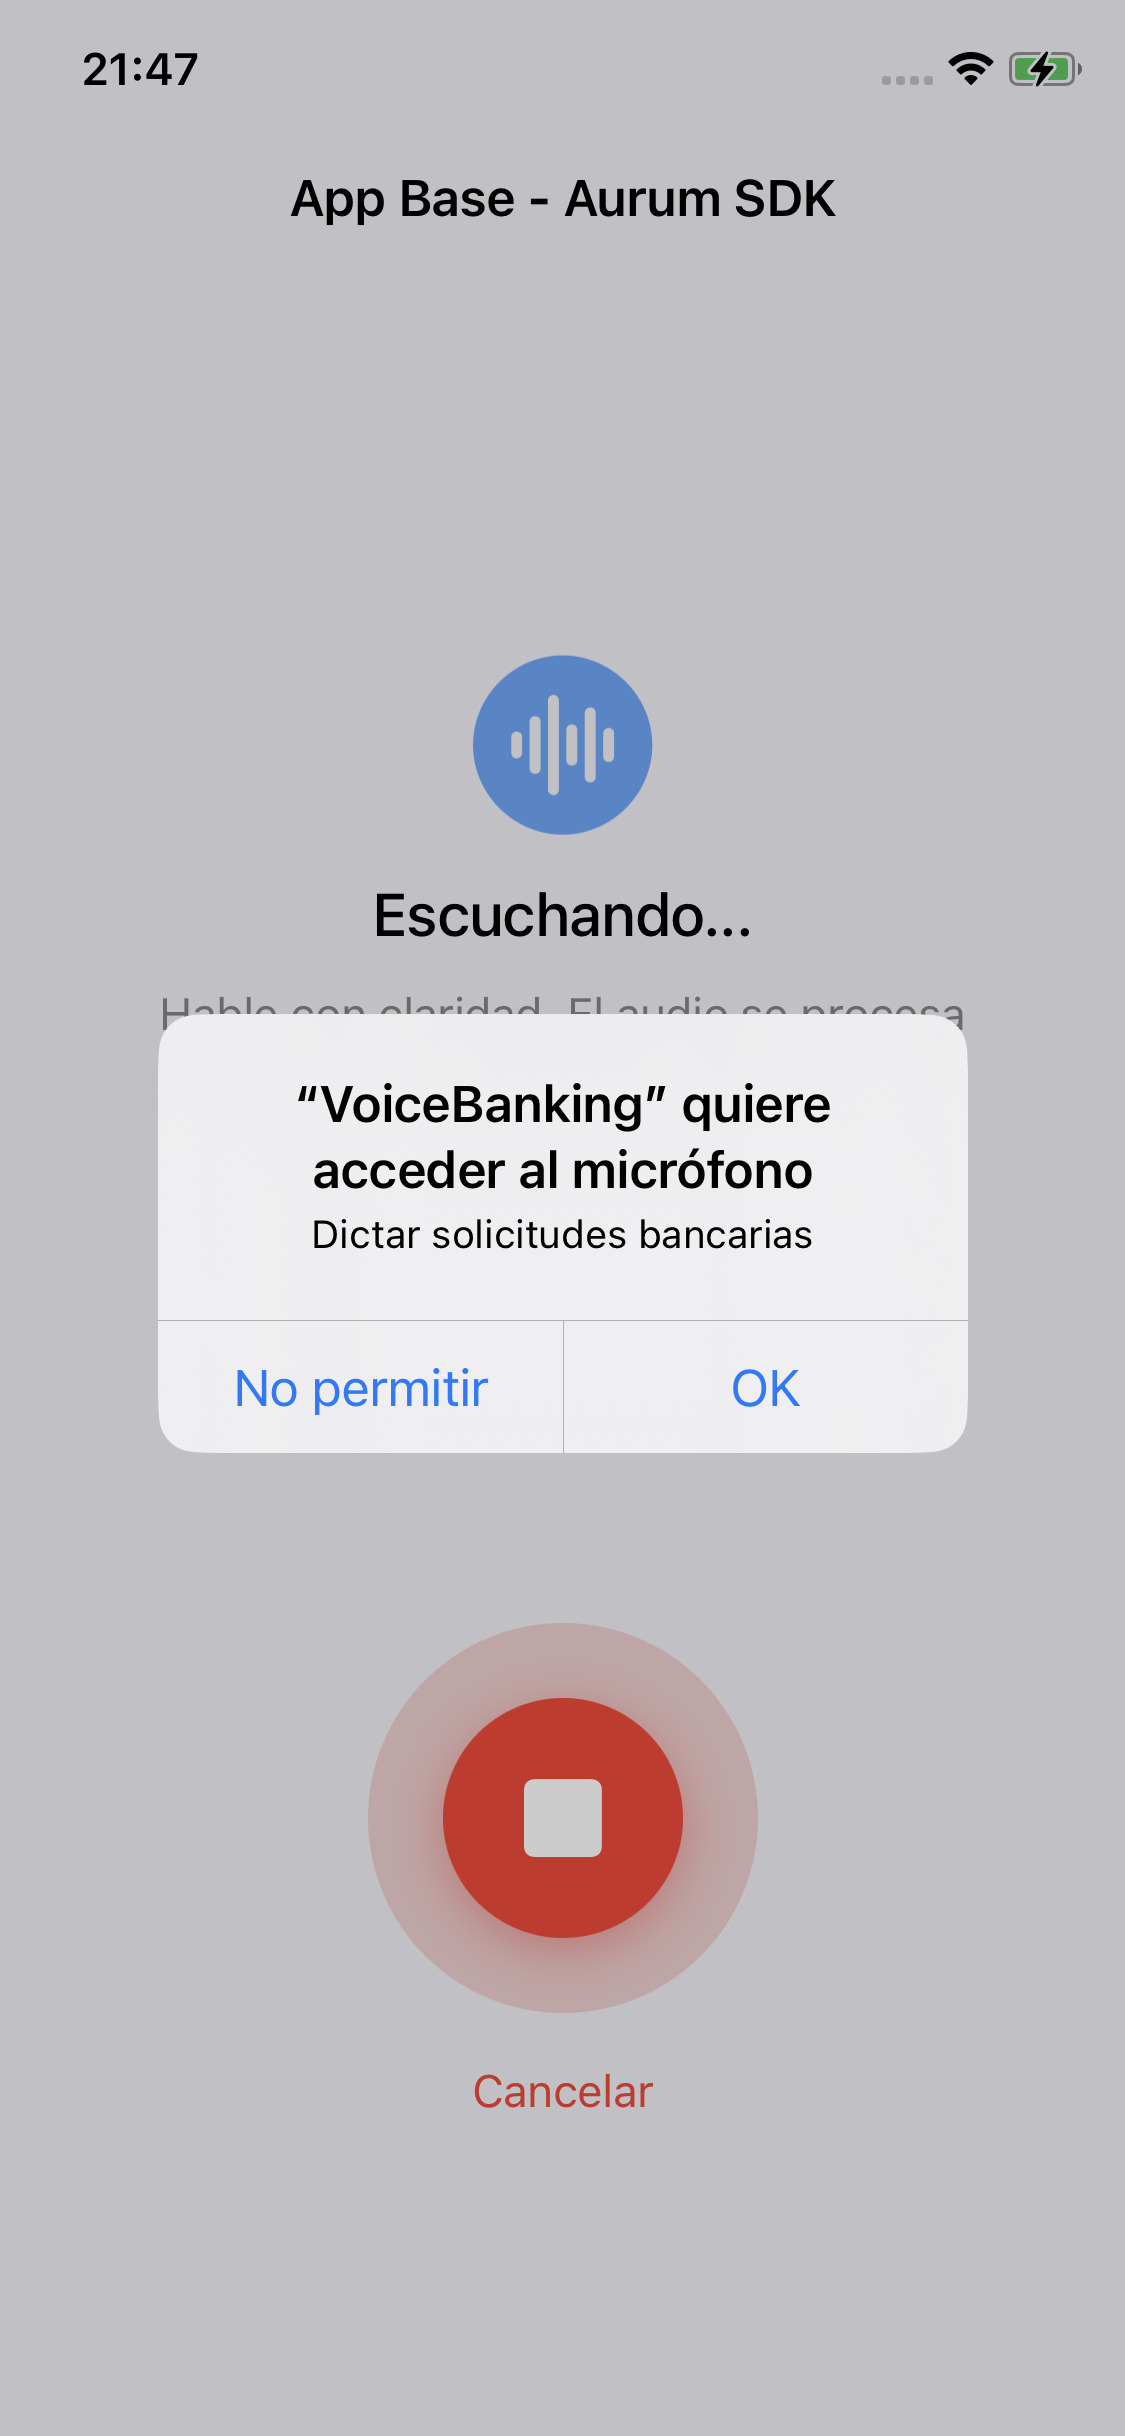
\includegraphics[width=0.65\textwidth]{./Figures/screenshots/solicitud-permiso-microfono.PNG}
         \caption[Solicitud de permiso de acceso al micrófono]{Permiso para uso del micrófono.}
         \label{fig:permiso-mic}
     \end{subfigure}
     \hfill
     \begin{subfigure}[b]{0.5\textwidth}
         \centering
         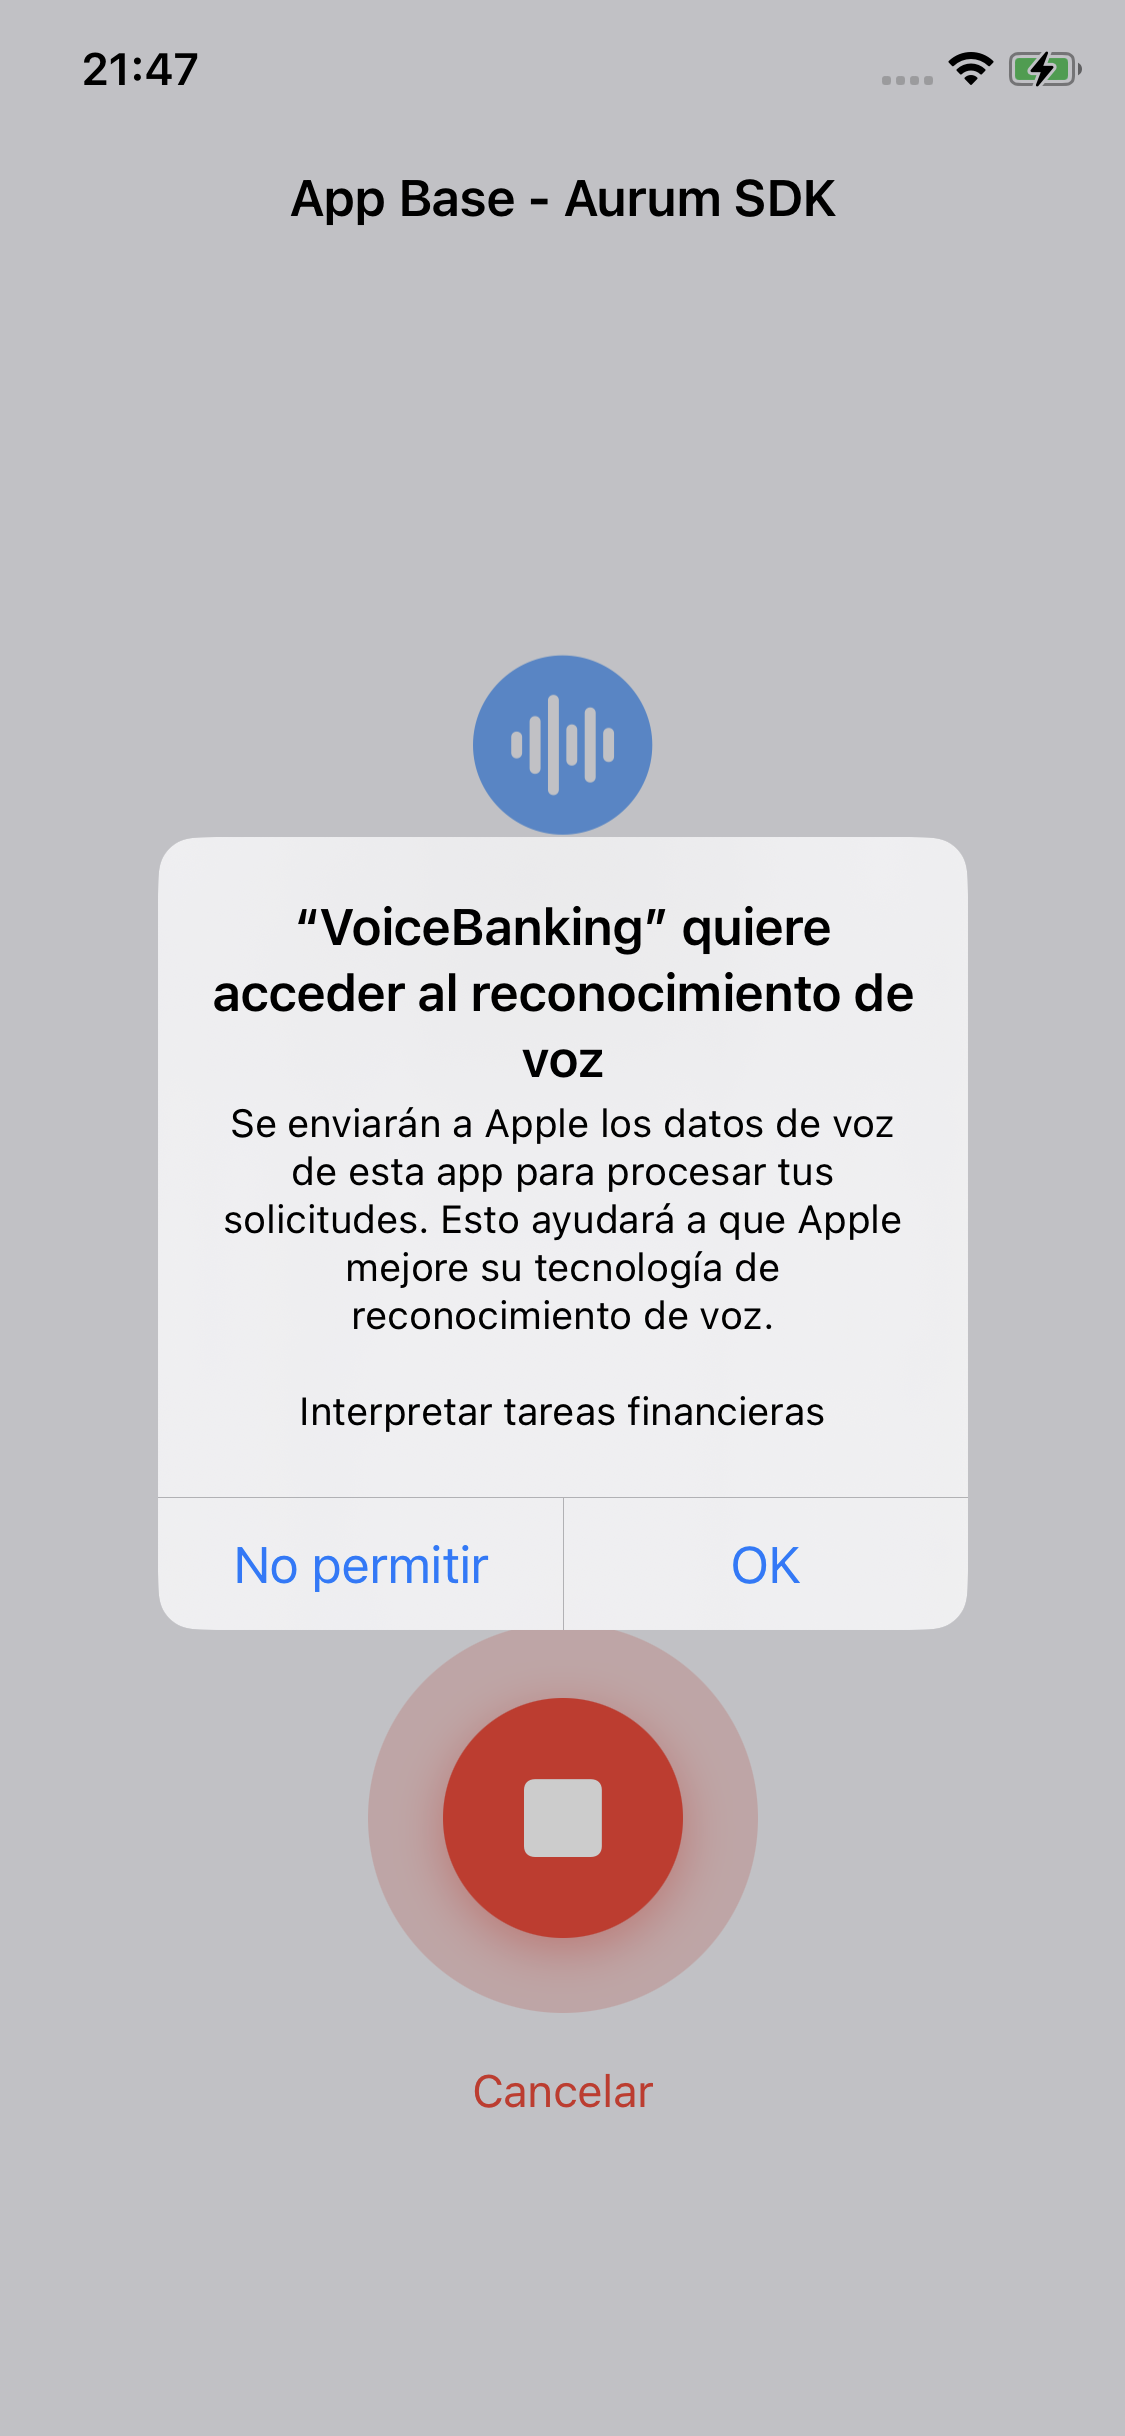
\includegraphics[width=0.65\textwidth]{./Figures/screenshots/solicitud-permiso-reconocimiento-voz.PNG}
         \caption[Solicitud de permiso de reconocimiento de voz]{Permiso para el reconocimiento de voz.}
         \label{fig:permiso-speech}
     \end{subfigure}
        \caption{Capturas de pantalla de las solicitudes de permisos en la aplicación base.}
        \label{fig:initial-state}
\end{figure}

Para cada tarea, se registraron las siguientes métricas:

\begin{itemize}
    \item Tasa de éxito: proporción de intentos en los que el sistema detectó correctamente la intención y las entidades, y el usuario pudo
    completar (o cancelar) la operación satisfactoriamente.

    \item Tiempo de interacción: tiempo transcurrido desde que el usuario presiona el botón de micrófono hasta que confirma o cancela en la
    pantalla de confirmación.

    \item Errores de interacción: cantidad de veces que el usuario necesitó reiniciar el comando (por ejemplo, porque habló antes de que el
    sistema estuviera escuchando, o porque no entendió el estado de la interfaz).
\end{itemize}


La figura ~\ref{fig:app-idle} ilustra el estado inicial de la interfaz en la applicación base. El botón azul con ícono de micrófono indica que el sistema está listo para recibir un comando de voz.

\begin{figure}[H]
	\centering
	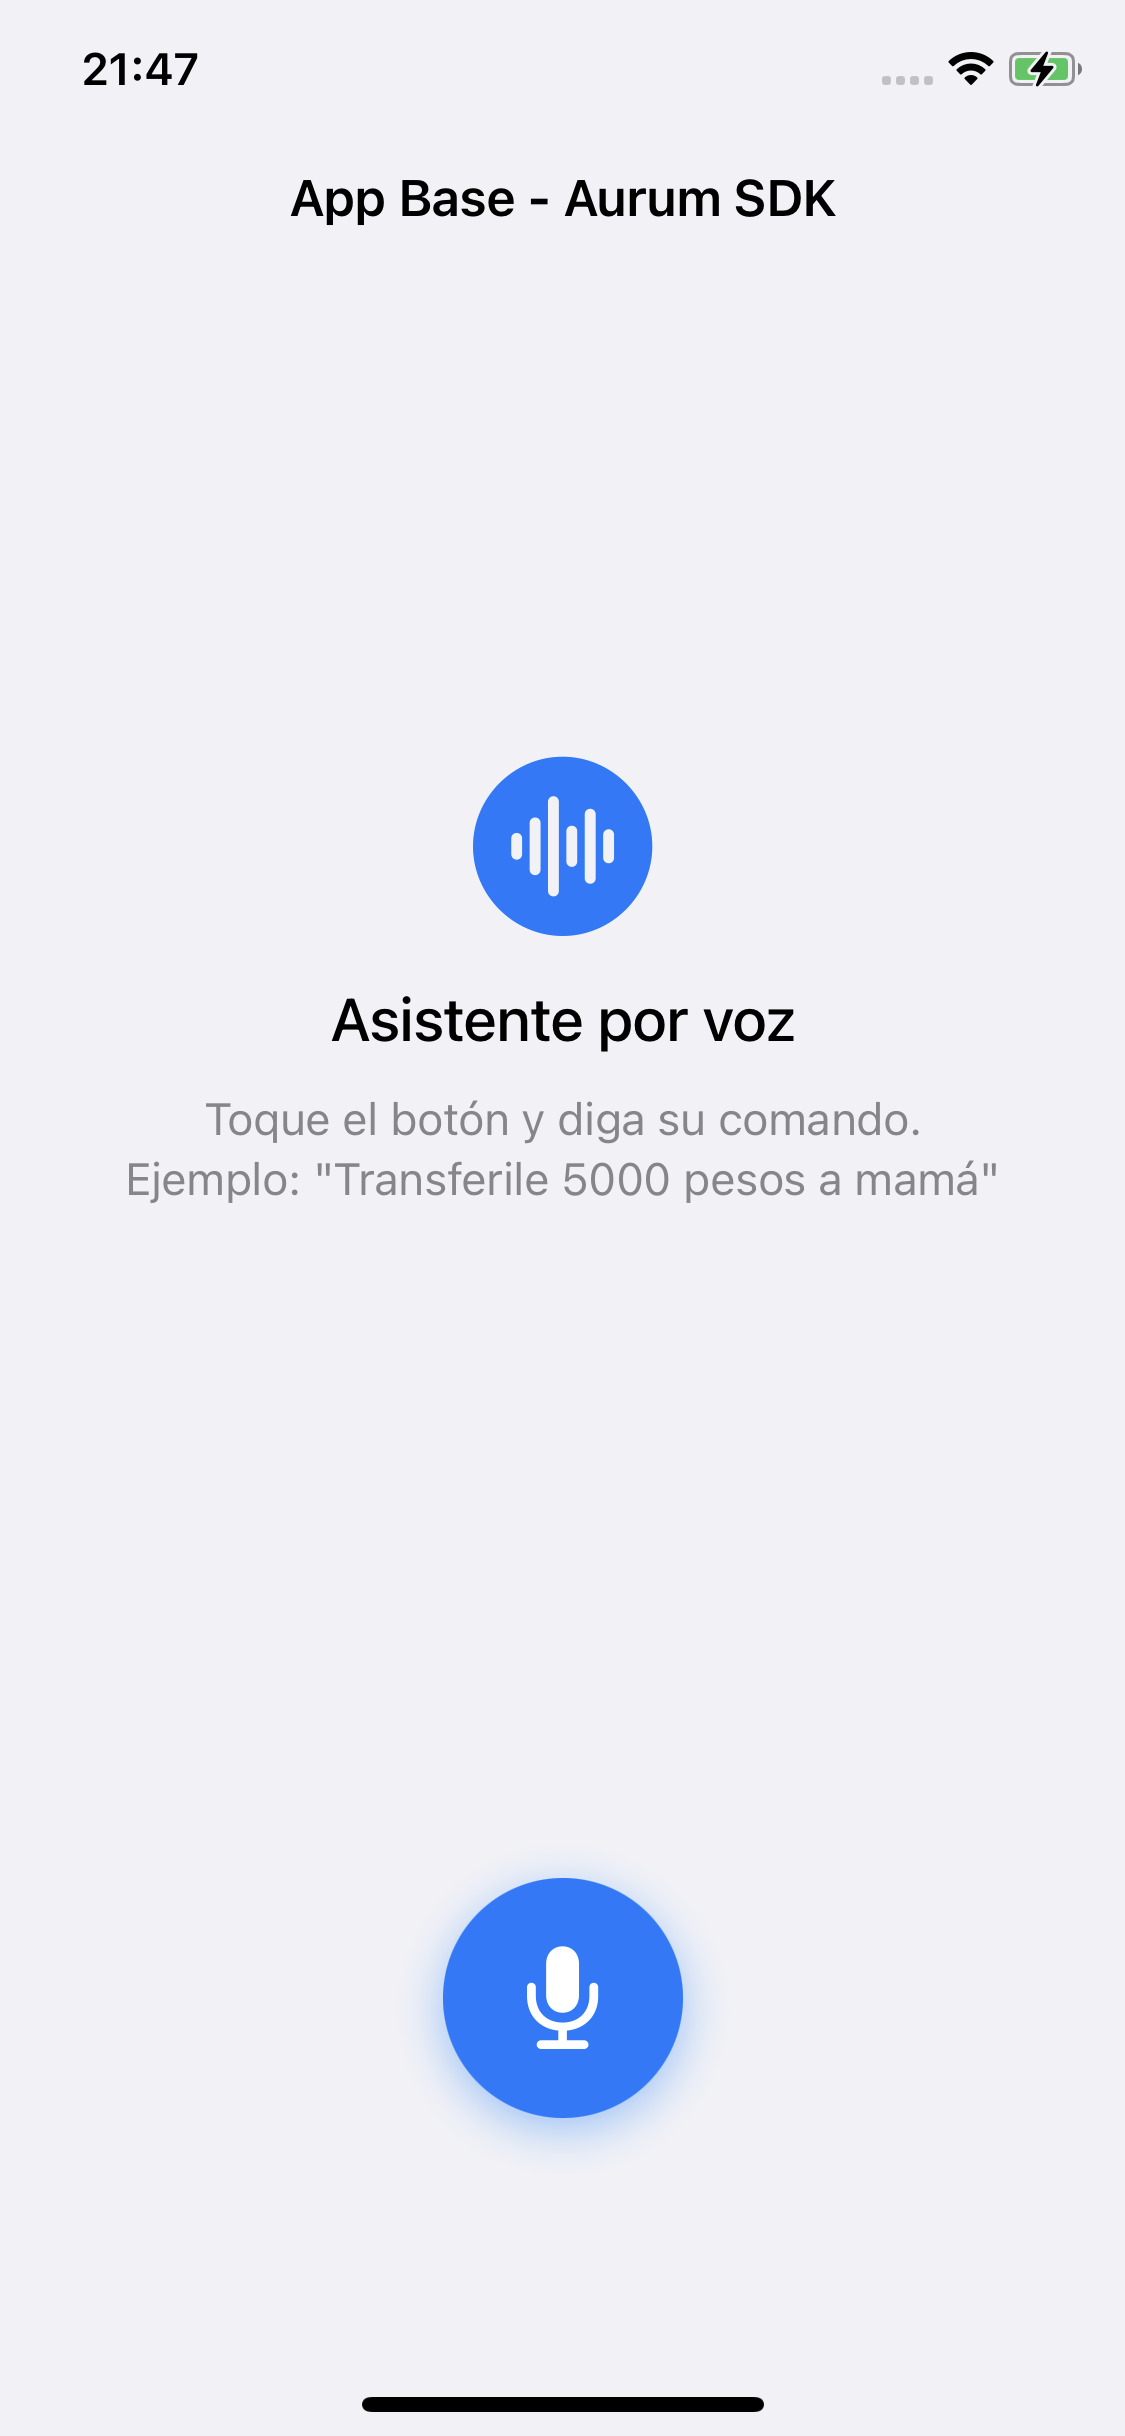
\includegraphics[width=0.75\textwidth]{./Figures/screenshots/home-app-base.PNG}
	\caption[Pantalla principal de la aplicación base en estado idle]{Pantalla principal de la aplicación base en estado \texttt{idle}. El botón azul con ícono de micrófono indica que el sistema está listo para recibir un comando de voz.}
	\label{fig:app-idle}
\end{figure}


En la figura ~\ref{fig:app-listening} se observa como se transcribe el audio en tiempo real y en ~\ref{fig:app-processing} se muestra el procesamiento del texto.

\begin{figure}[!htpb]
     \begin{subfigure}[b]{0.45\textwidth}
         \centering
         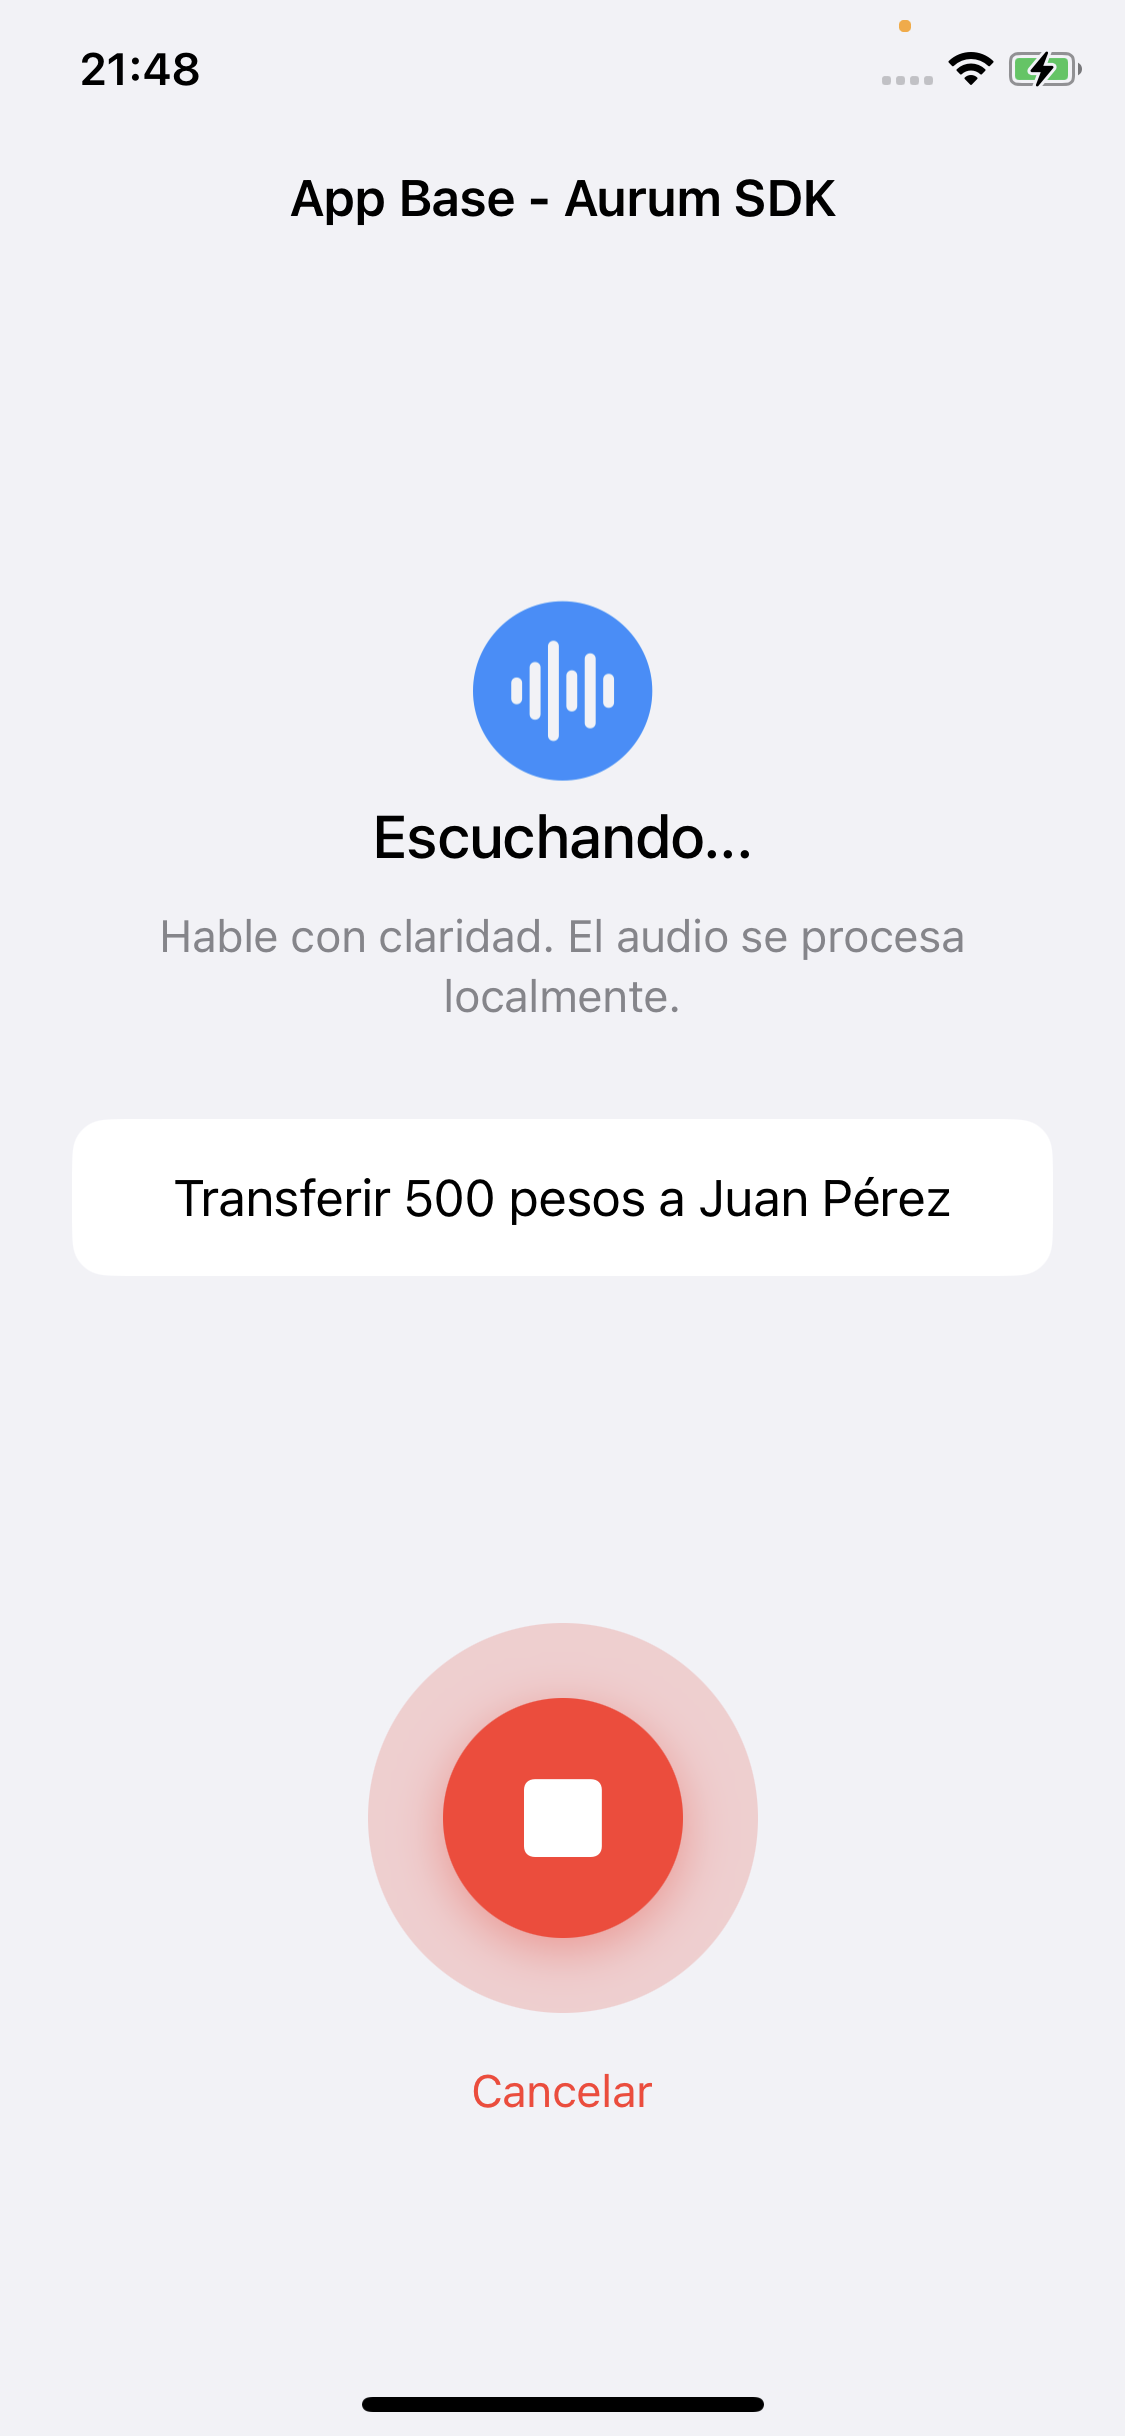
\includegraphics[width=0.85\textwidth]{./Figures/screenshots/transcripcion-dictado.PNG}
         \caption[Estado escuchando]{Estado \texttt{listening}: La transcripción parcial se muestra en tiempo real.}
         \label{fig:app-listening}
     \end{subfigure}
     \hfill
     \begin{subfigure}[b]{0.45\textwidth}
         \centering
         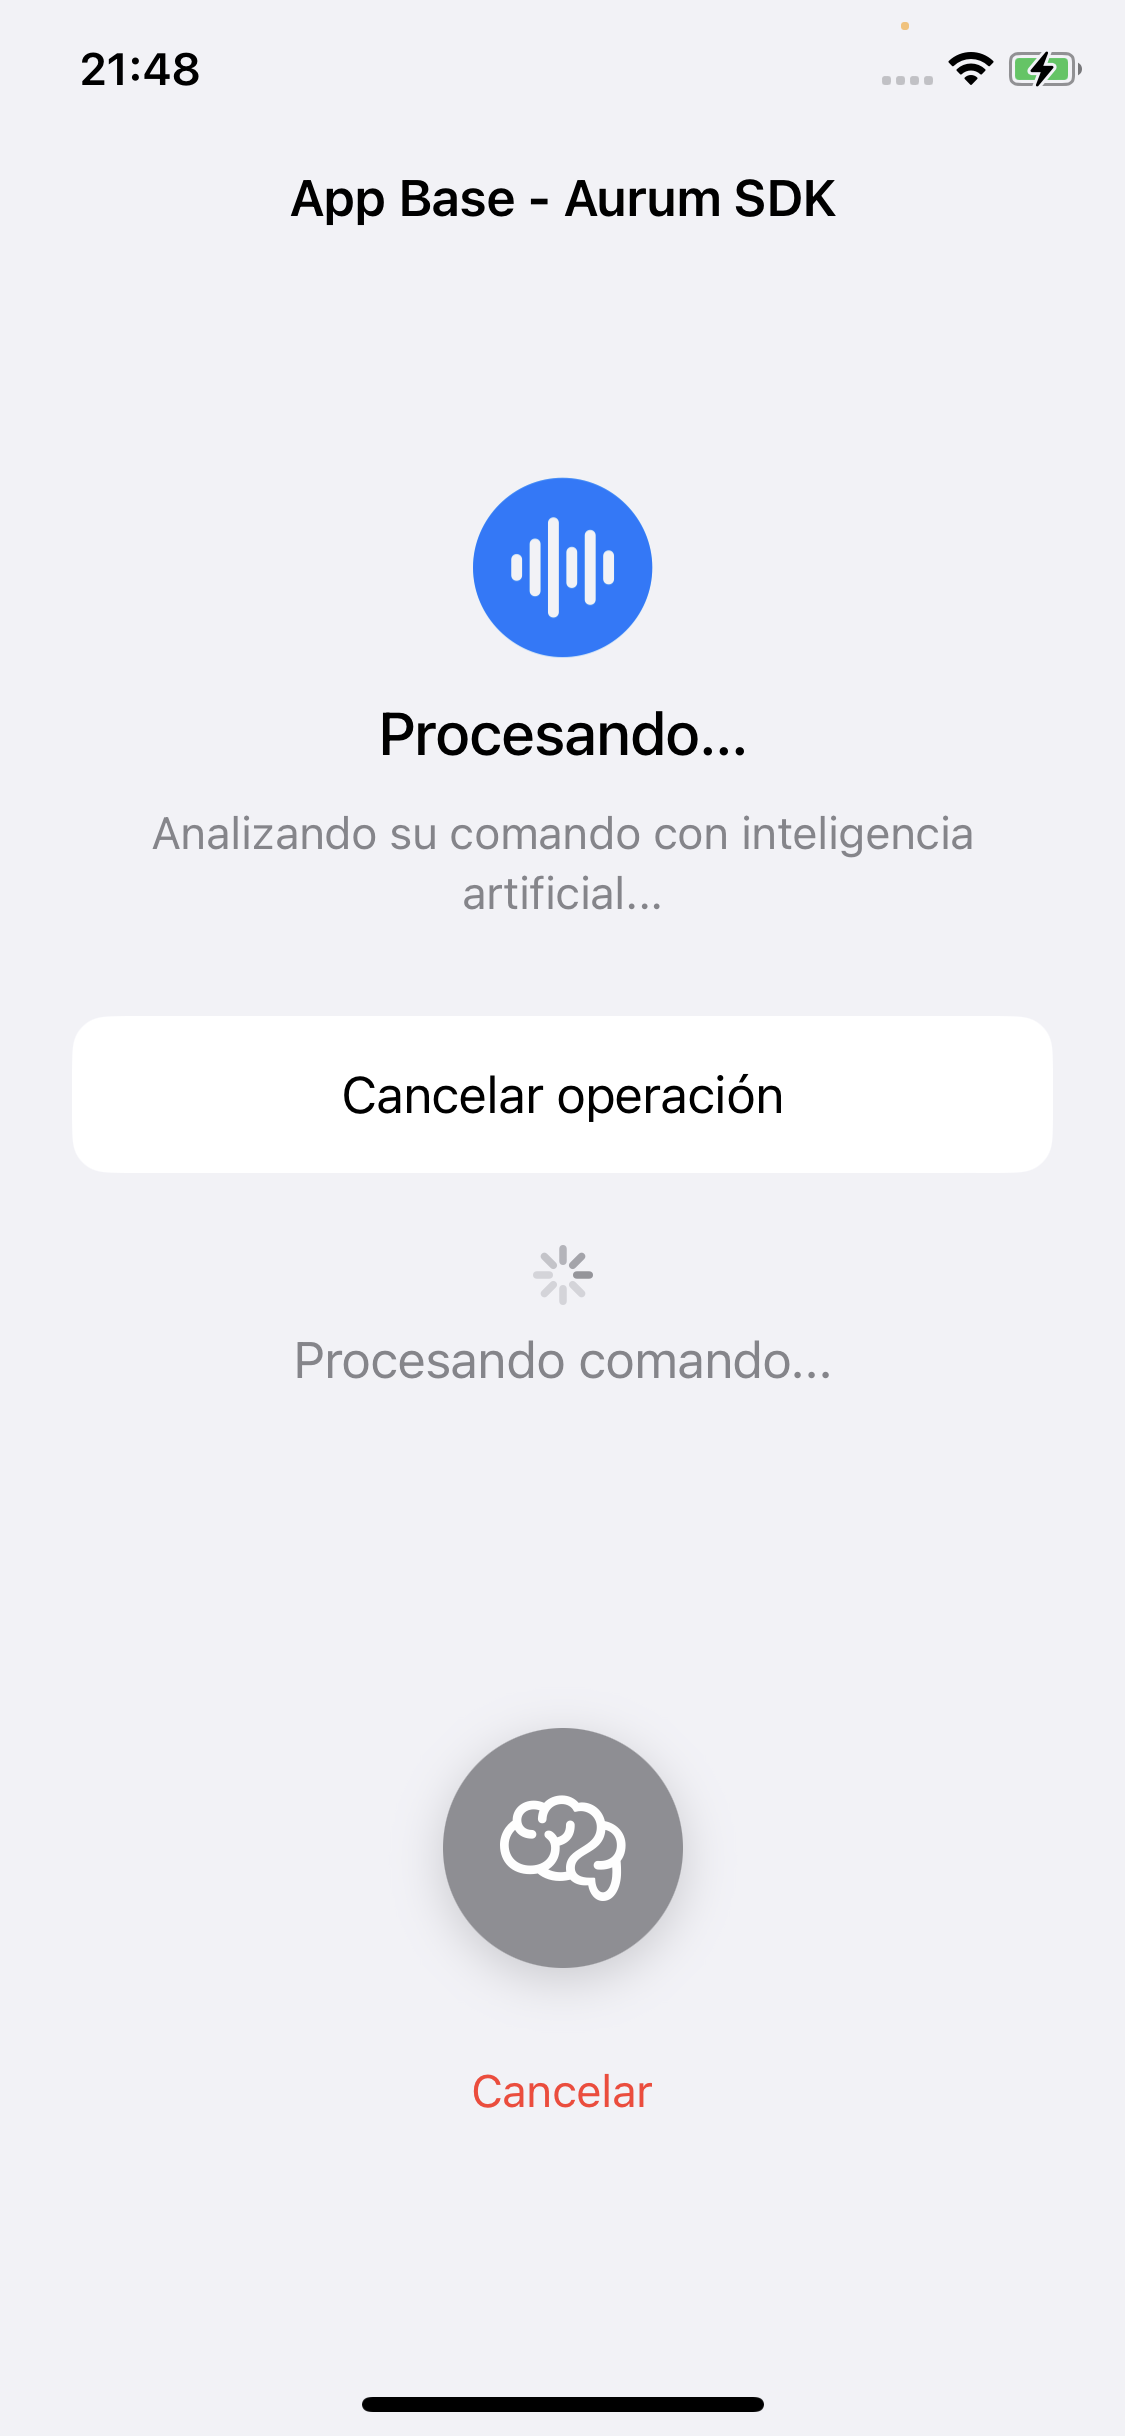
\includegraphics[width=0.85\textwidth]{./Figures/screenshots/procesamiento.PNG}
         \caption[Estado procesando audio a texto]{Estado \texttt{processing}: en este punto los modelos Core~ML ejecutan la inferencia.}
         \label{fig:app-processing}
     \end{subfigure}
        \caption{Capturas de pantalla que ilustran el funcionamiento de la transcripción en tiempo real y el procesamiento a texto.}
        \label{fig:working-state}
\end{figure}


\subsection{Resultados de usabilidad}
\label{subsec:resultados-usabilidad}

Los resultados de las pruebas de usabilidad arrojan las siguientes
observaciones:

\subsubsection*{Retroalimentación visual de la transcripción}

La visualización en tiempo real de la transcripción parcial en la \texttt{MainView} fue percibida como un elemento positivo de la experiencia.
La presencia de texto que se actualiza progresivamente mientras el usuario habla genera confianza en que el sistema está procesando activamente el comando, reduciendo la incertidumbre inherente a la interacción con sistemas de voz. En as tareas donde la transcripción mostró errores visibles (por ejemplo, en T2 cuando el reconocedor transcribió \texttt{luca} como \texttt{luca} sin convertirlo), los usuarios pudieron anticipar un posible error antes de ver la pantalla de confirmación.

\subsubsection*{Pantalla de confirmación}

El paso de confirmación obligatorio fue valorado positivamente en el contexto financiero. Los usuarios expresaron mayor confianza al poder verificar
visualmente el monto, la moneda y el destinatario antes de confirmar la operación. La presentación desglosada del \texttt{TransactionPayload}, especialmente el campo de \texttt{confianza} expresado como porcentaje, permitió a los usuarios evaluar la certeza del sistema y decidir de manera informada si confirmar o reintentar el comando.

La figura ~\ref{fig:confirm-transferencia} muestra la pantalla de confirmación de una transferencia detectada.

\begin{figure}[H]
	\centering
	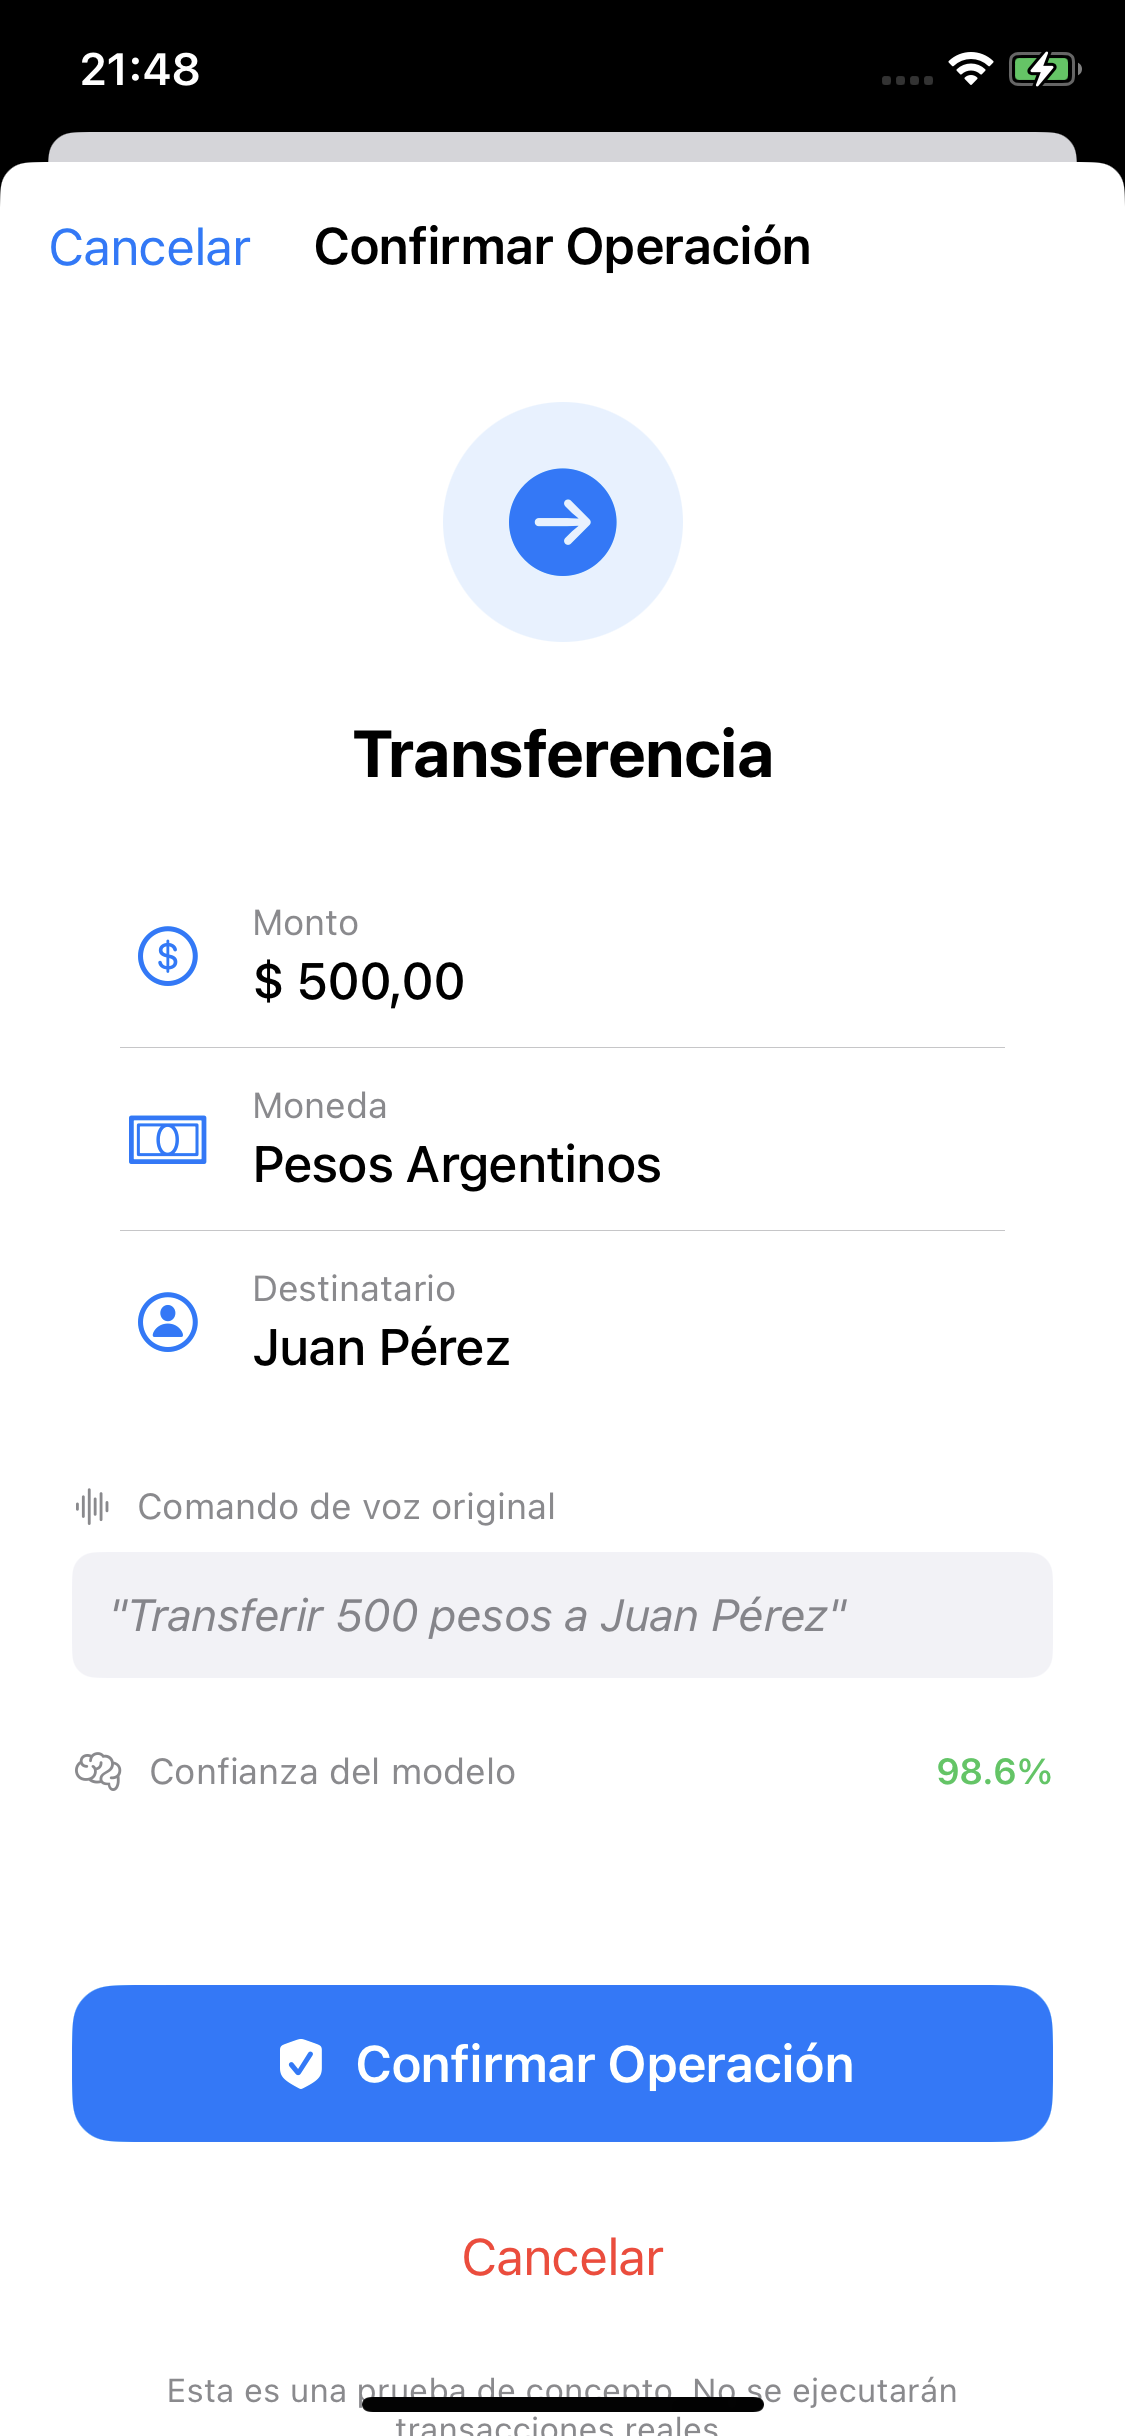
\includegraphics[width=0.35\textwidth]{./Figures/screenshots/intencion-confirmacion-transferencia.PNG}
	\caption[Pantalla de confirmación de transferencia]{Pantalla de confirmación para una transferencia exitosa. Se muestra el monto (\$~500,00), la moneda (Pesos Argentinos), el destinatario (Juan Pérez), la transcripción original y la confianza del modelo (98,6\%).}
	\label{fig:confirm-transferencia}
\end{figure}

La figura ~\ref{fig:confirm-saldo} muestra la pantalla de confirmación de una consulta de saldo.

\begin{figure}[H]
	\centering
	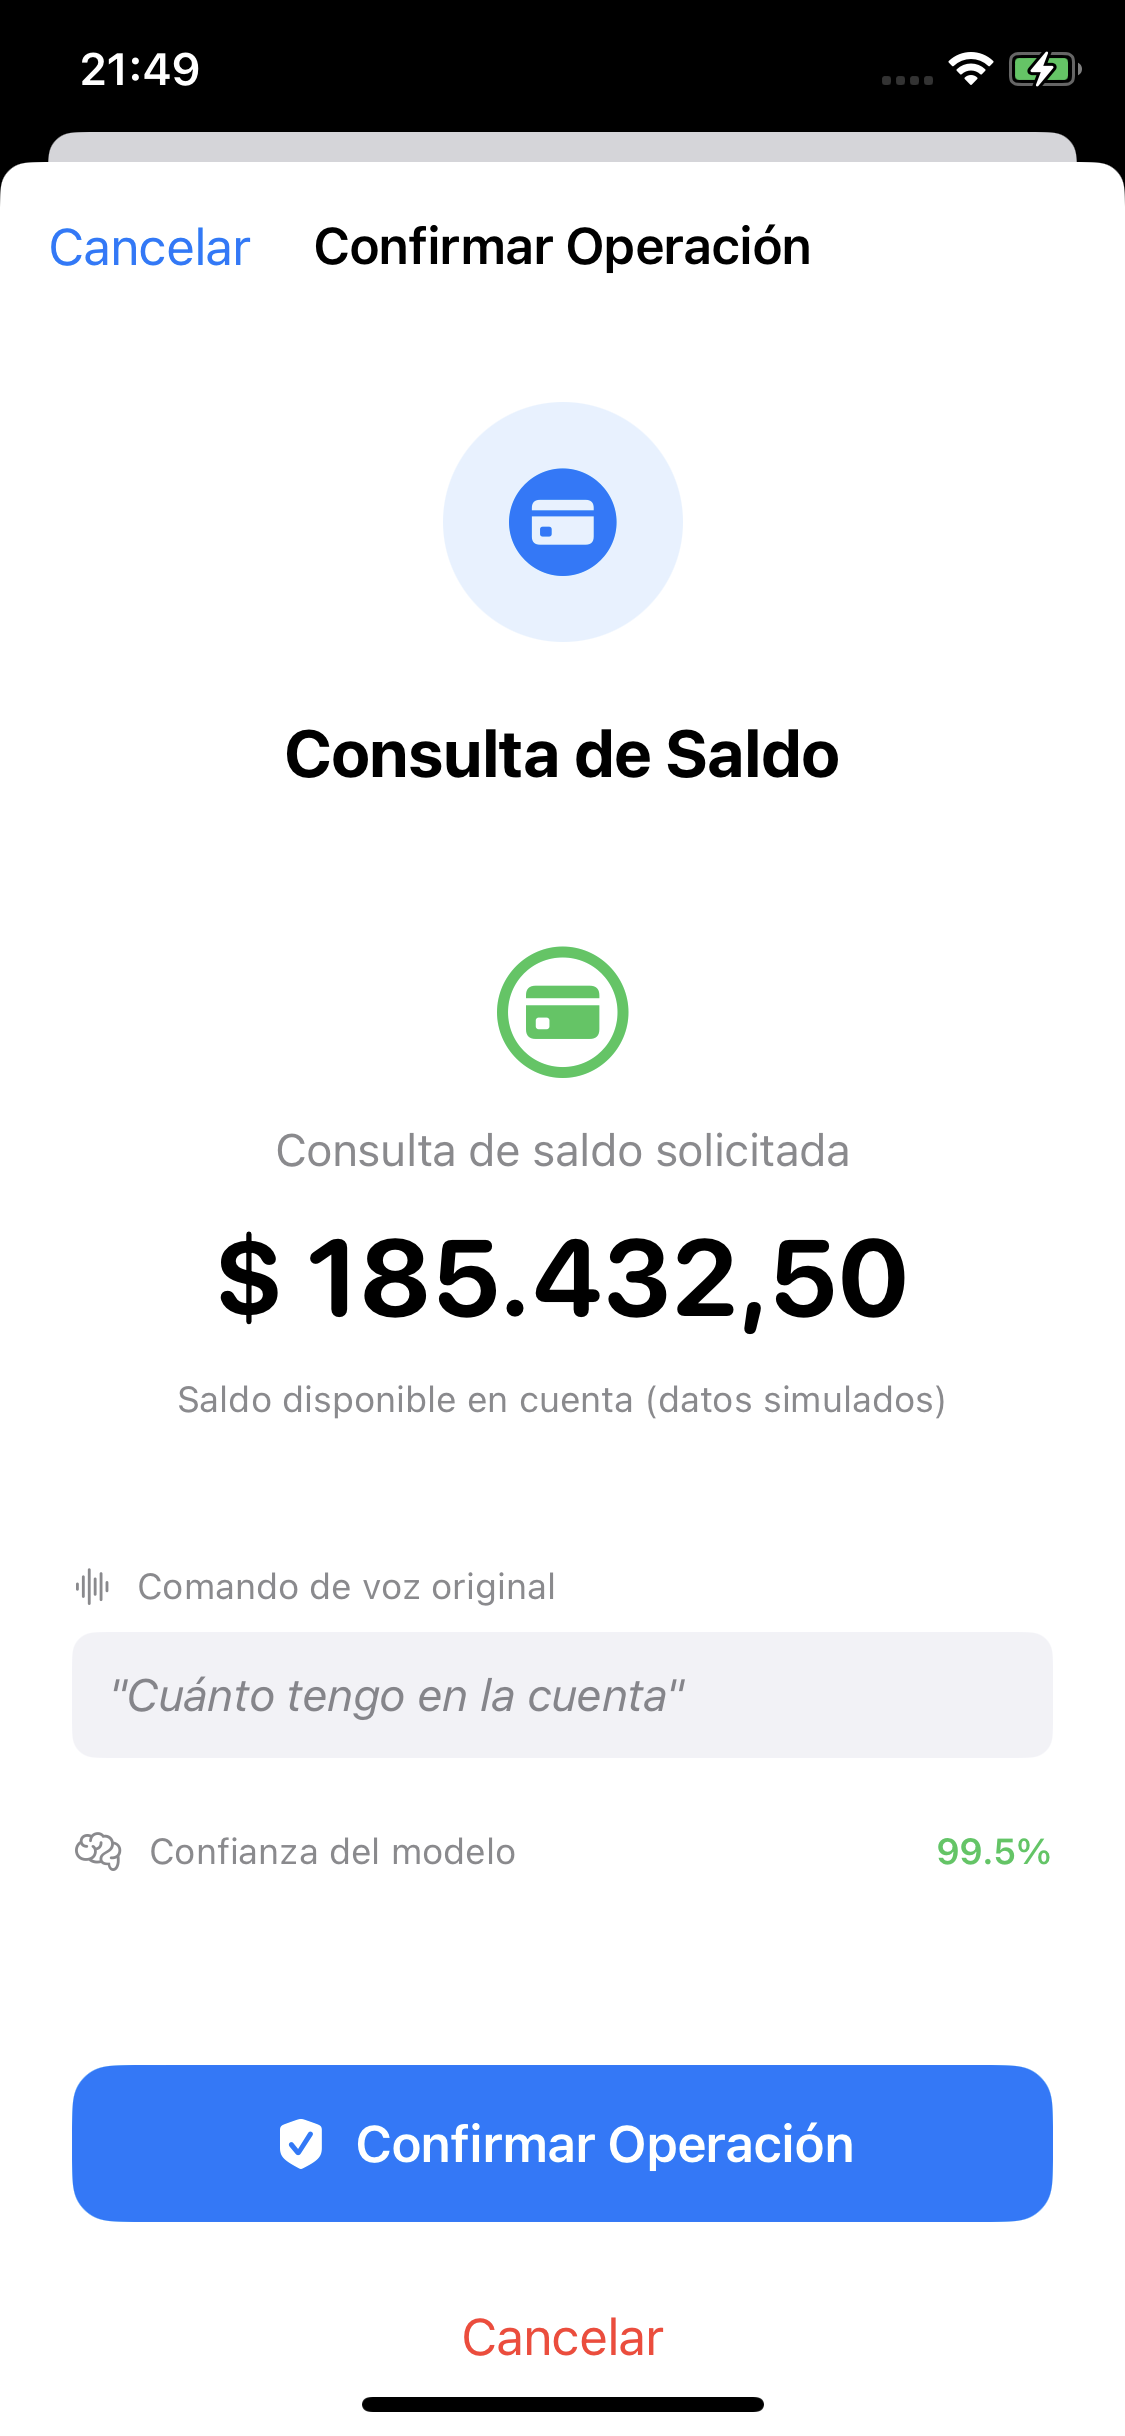
\includegraphics[width=0.45\textwidth]{./Figures/screenshots/intencion-consulta-saldo.PNG}
	\caption[Confirmación de consulta de saldo]{Confirmación de consulta de saldo. Se presenta el saldo simulado y la confianza del modelo (99,5\%).}
	\label{fig:confirm-saldo}
\end{figure}

La figura ~\ref{fig:confirm-cancelar} muestra la pantalla de confirmación de una anulación o cancelación de operación.

\begin{figure}[H]
	\centering
	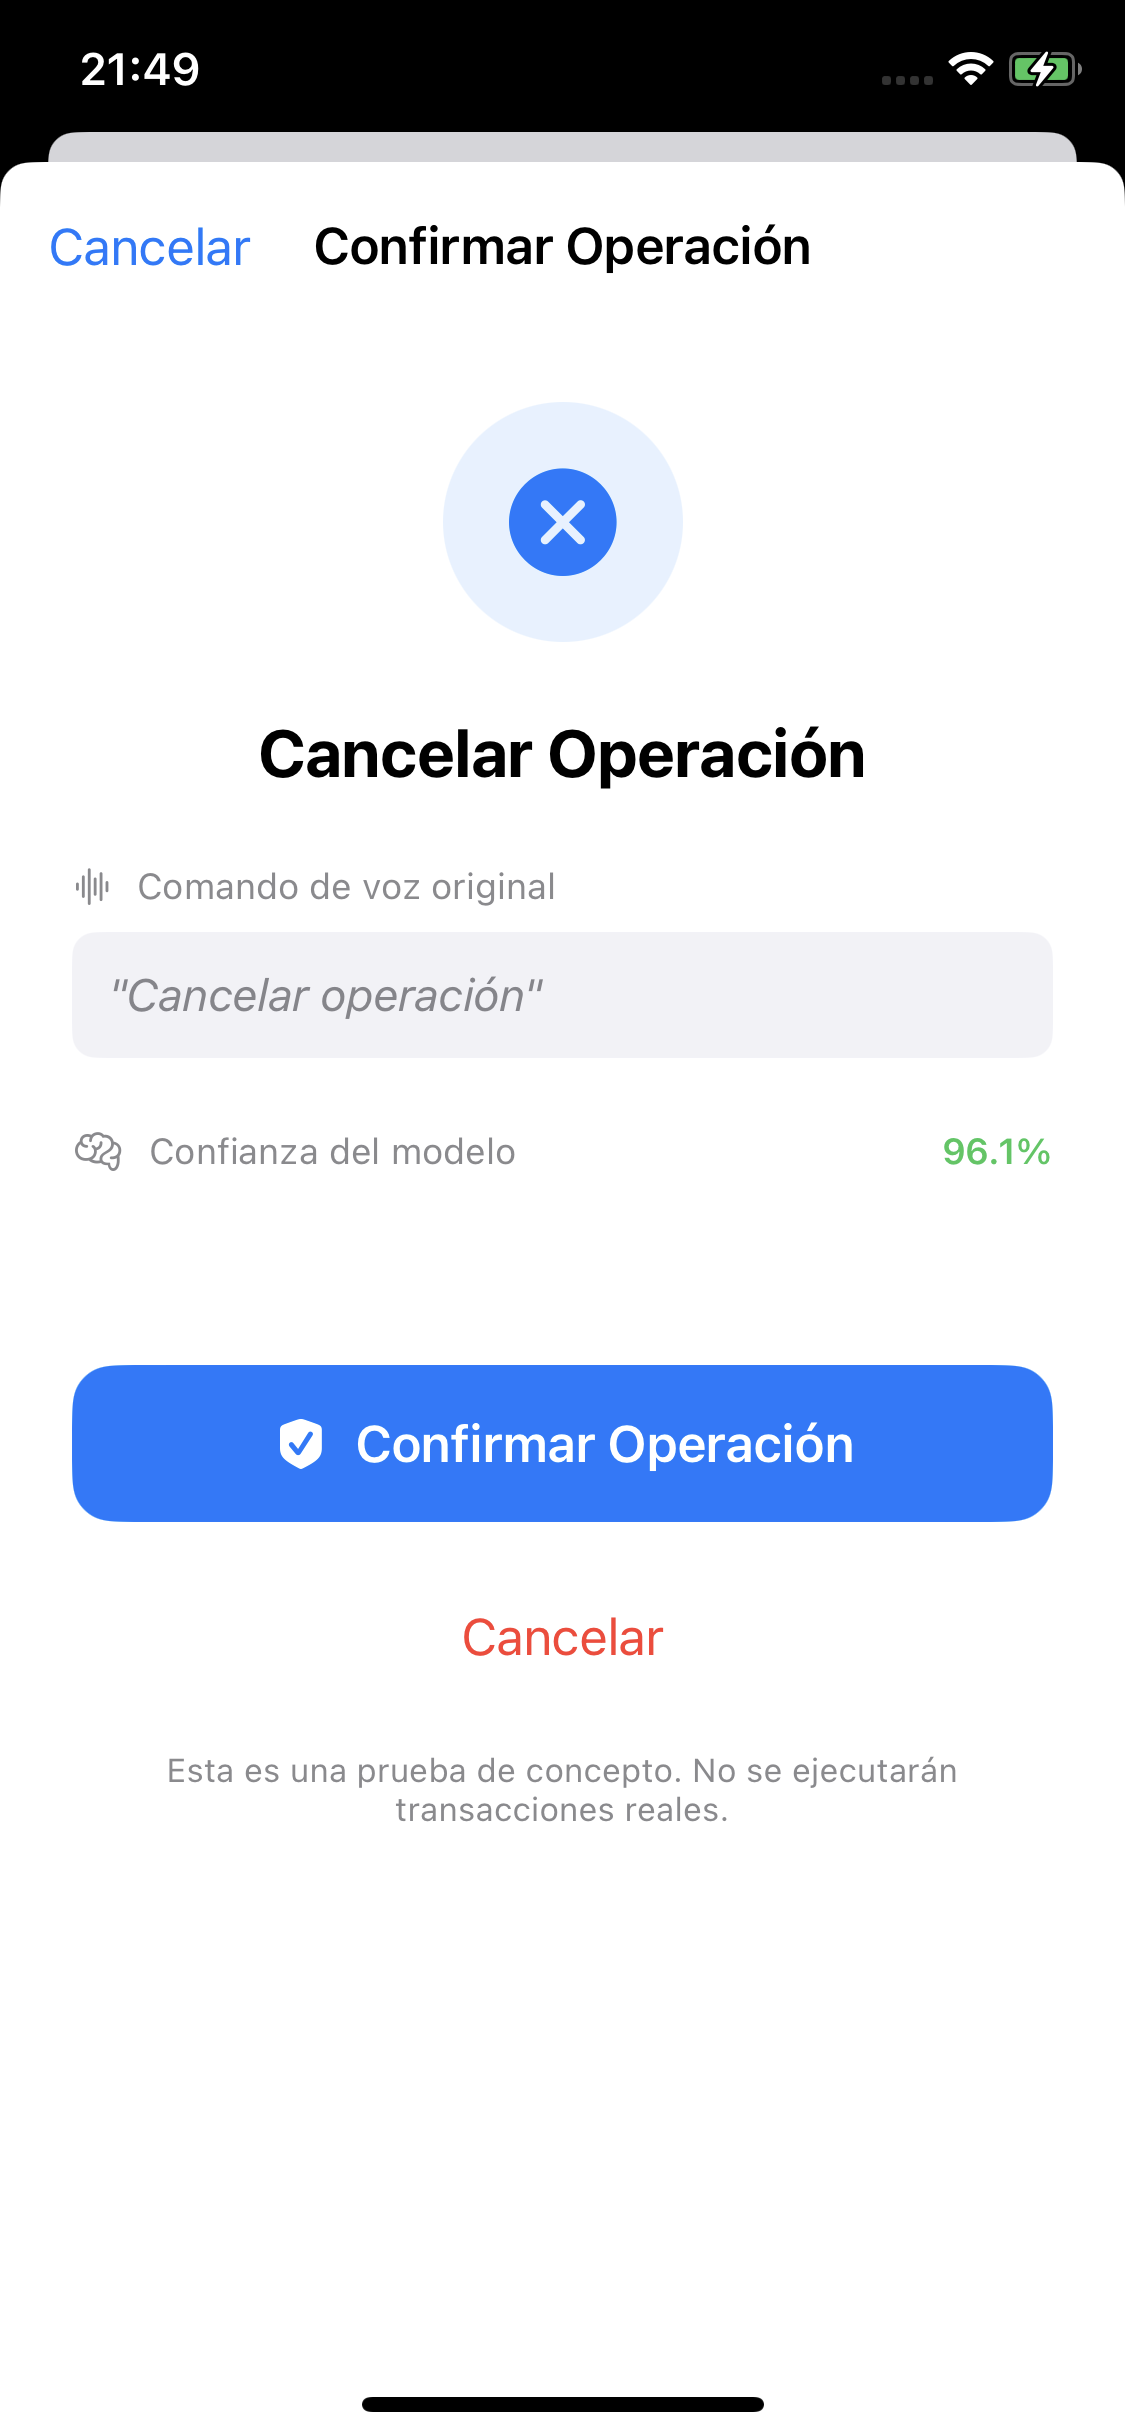
\includegraphics[width=0.45\textwidth]{./Figures/screenshots/intencion-cancelar.PNG}
	\caption[Confirmación de intención de cancelación]{Confirmación de intención de cancelación. El modelo clasificó el comando con una confianza de 96,1\%.}
	\label{fig:confirm-cancelar}
\end{figure}


\subsubsection*{Latencia percibida}

El tiempo transcurrido entre el fin del habla y la aparición de la pantalla de confirmación fue percibido como instantáneo en la mayoría de las tareas.
Esto es consistente con las mediciones de latencia reportadas en la sección~\ref{subsec:latencia}: el procesamiento NLU se completa en el orden de
los milisegundos, y la latencia dominante corresponde al \textit{Speech Framework}, que opera en modo \textit{streaming} y entrega la transcripción
final con un retardo del orden de 100--300~ms tras el último \textit{buffer} de audio.

\subsubsection*{Tarea ambigua (T6)}

La tarea T6 (\texttt{anular la transferencia de ayer}) fue incluida deliberadamente para evaluar el comportamiento del sistema ante un comando fuera del espacio de capacidades soportadas. La referencia temporal \texttt{de ayer} no es una entidad modelada, y la mezcla de \texttt{anular} con \texttt{transferencia} introduce ambigüedad entre las intenciones \textsc{cancelar} y \textsc{transferencia}. El comportamiento observado fue que el modelo clasificó el comando con una confianza inferior al umbral de 0,65, asignando la intención \texttt{.desconocida}. La aplicación base presentó un mensaje indicando que no pudo interpretar el comando, invitando al usuario a reformularlo. Este comportamiento es el deseado: el sistema prefiere rechazar un comando ambiguo
antes que ejecutar una operación financiera potencialmente incorrecta.

En la siguiente tabla ~\ref{tab:usabilidad} se ven reflejados los resultados de las pruebas realizadas:

% --- TABLA: Resultados de usabilidad ---
\begin{table}[H]
\caption{Resultados de las pruebas de usabilidad por tarea. La tasa de éxito
         se calcula sobre el total de intentos. El tiempo de interacción incluye
         el habla del usuario, el procesamiento y la confirmación.}

\centering
\label{tab:usabilidad}
\begin{tabular}{@{}lcccc@{}}
\toprule
\textbf{Tarea}
  & \textbf{Tasa de éxito}
  & \textbf{Tiempo medio}
  & \textbf{Errores}
  & \textbf{Intentos} \\
\midrule
T1 --- Transf. estándar   & 100\%  & 4,4 s & 0,0 & 1,0 \\
T2 --- Transf. coloquial  & 80\%   & 3,7 s & 0,6 & 1,8 \\
T3 --- Transf. dólares    & 100\%  & 3,9 s & 0,2 & 2,4 \\
T4 --- Consulta de saldo  & 100\%  & 3,3 s & 0,0 & 1,0 \\
T5 --- Cancelación        & 100\%  & 5,0 s & 0,0 & 3,2 \\
T6 --- Comando ambiguo    & 0\%    & 4,9 s & 3,4 & 3,4 \\
\midrule
\textit{Promedio}         & 80\%   & 4,2 s & 0,7 & --- \\
\bottomrule
\end{tabular}
\end{table}



% =============================================================================
% 4.4 ANÁLISIS DE RESULTADOS
% =============================================================================

\section{Análisis de resultados}
\label{sec:analisis}

Esta sección integra los resultados experimentales presentados en las secciones anteriores, los contrasta con el marco teórico establecido en el capítulo~2, y discute las implicancias para la viabilidad técnica de la solución propuesta.


\subsection{Validación de la hipótesis central}
\label{subsec:validacion-hipotesis}

La hipótesis central de este trabajo sostiene que es posible resolver, de forma íntegra en el dispositivo móvil, el problema dual de clasificar intenciones y extraer entidades nombradas a partir de comandos de voz financieros, utilizando exclusivamente los \textit{frameworks} nativos de Apple: Create~ML para el entrenamiento de modelos (MaxEnt para clasificación, CRF para etiquetado de secuencias) y los \textit{frameworks} \texttt{NaturalLanguage} y Core~ML para la inferencia local.

Los resultados obtenidos respaldan esta hipótesis. El clasificador de intenciones alcanzó un Macro F1-Score de 1,00 sobre el conjunto de test,
un valor que indica una capacidad discriminativa alta para las tres clases definidas. El extractor de entidades logró un Entity F1 \textit{strict} macro de 0,9369, que si bien es inferior al del clasificador, lo que es esperable dado que la extracción de entidades es intrínsecamente una tarea más compleja que la clasificación de texto, resulta suficiente para la prueba de concepto
propuesta.


\subsection{Comparación con arquitecturas alternativas}
\label{subsec:comparacion-arquitecturas}

La comparativa de arquitecturas presentada en el capítulo teórico estableció una comparación cualitativa entre tres familias de
arquitecturas: Transformers (BETO), redes recurrentes (BiLSTM) y frameworks nativos de Apple (Create~ML). Los resultados experimentales permiten ahora complementar esa comparación con evidencia cuantitativa.

En términos de precisión predictiva, la literatura reporta que modelos basados en BETO alcanzan F1-Scores del orden de 0,95--0,98 para clasificación de
intenciones en español \citep{canete2020spanish}, y que las arquitecturas BiLSTM-CRF obtienen valores de 0,88--0,93 para NER en dominios específicos \citep{lample2016neural}. Los valores obtenidos con Create~ML se ubican en un rango competitivo con los reportados para BiLSTM, aunque ligeramente inferiores a los de BETO.

Sin embargo, la comparación de precisión aislada es insuficiente. El análisis debe ponderarse con las restricciones operativas del \textit{edge computing}:

\begin{itemize}
    \item Tamaño del modelo: los modelos Create~ML ocupan menos de 1~MB en disco, frente a los $\sim$440~MB de BETO y los $\sim$5--15~MB de
    un BiLSTM. Para un dispositivo móvil con almacenamiento limitado y donde la aplicación bancaria compite por espacio con otras aplicaciones, esta
    diferencia de dos a tres órdenes de magnitud es determinante.

    \item Latencia de inferencia: los modelos nativos resolvieron el \textit{pipeline} completo en menos de 1~ms promedio. Un BETO sin comprimir
    requiere típicamente más de 200~ms por inferencia en un dispositivo móvil \citep{sun2020mobilebert}, lo que acumularía una latencia perceptible al
    ejecutar las dos inferencias (clasificación + NER) en secuencia.

    \item Integración nativa: los modelos Create~ML no requieren conversión con \texttt{coremltools} ni adaptaciones de formato. Se
    entrenan en macOS, se generan como \texttt{.mlmodel}, y Xcode los compila automáticamente a \texttt{.mlmodelc} al integrarlos al proyecto. Esta
    cadena de herramientas cerrada elimina una fuente significativa de errores de integración y mantenimiento.

    \item Privacidad nativa: al operar exclusivamente con frameworks de Apple, el sistema hereda las garantías de privacidad del ecosistema iOS.
    No se requiere configuración adicional para asegurar que los datos no abandonen el dispositivo, a diferencia de las arquitecturas basadas en
    PyTorch o TensorFlow que requieren validación explícita de que la inferencia se ejecuta localmente.
\end{itemize}

En síntesis, la pérdida marginal de precisión respecto a BETO se compensa con ventajas sustanciales en tamaño, latencia, facilidad de integración y
garantías de privacidad. Para el caso de uso específico de una prueba de concepto en el sector financiero argentino, donde la privacidad y la
latencia son requisitos no negociables, el \textit{trade-off} resulta favorable a la arquitectura nativa.


\subsection{Rol del \texttt{TextNormalizer}}
\label{subsec:rol-normalizer}

Los ensayos de robustez (tabla~\ref{tab:robustez}) evidencian el impacto crítico del componente \texttt{TextNormalizer} en el rendimiento del sistema.
Las categorías de coloquialismos y expresiones numéricas presentan una degradación moderada respecto a la línea base, lo que indica que el normalizador logra convertir una proporción significativa de las variaciones léxicas a formas canónicas que los modelos pueden interpretar.

No obstante, la categoría de mezcla de variaciones, donde confluyen coloquialismos, errores de STT y expresiones numéricas, exhibe la mayor
caída de rendimiento. Esto sugiere que el normalizador basado en reglas determinísticas (diccionarios de equivalencias y patrones de expresiones
regulares) alcanza un techo de capacidad cuando las variaciones se acumulan. Un enfoque más robusto podría complementar las reglas con un modelo de corrección ortográfica o un \textit{spell checker} adaptado al dominio financiero, capaz de recuperar tokens distorsionados por errores de
transcripción.


\subsection{Limitaciones del estudio}
\label{subsec:limitaciones}

Es pertinente explicitar las limitaciones del presente trabajo, tanto para contextualizar adecuadamente los resultados como para orientar el trabajo
futuro:

\begin{enumerate}
    \item Corpus sintético: los modelos fueron entrenados y evaluados sobre un corpus generado mediante plantillas y aumentación de datos. Si
    bien esta estrategia permite controlar la distribución de clases y entidades, no captura la totalidad de la variabilidad lingüística del habla
    espontánea. Un corpus recolectado a partir de grabaciones de usuarios reales proporcionaría una evaluación más representativa.

    \item Dominio acotado: el sistema soporta únicamente tres intenciones y tres tipos de entidades. Una aplicación bancaria productiva
    requeriría un catálogo significativamente más amplio de operaciones (pagos de servicios, inversiones, consultas de movimientos, etc.) y entidades
    (fechas, números de cuenta, CBU/CVU).

    \item Idioma único: la implementación se centra exclusivamente en español rioplatense. Si bien el reconocedor de voz utiliza un mecanismo de \textit{fallback} que selecciona automáticamente el locale con soporte \textit{on-device} (\texttt{es-MX} o \texttt{es-ES}), los modelos NLU y el normalizador fueron entrenados y configurados para el léxico rioplatense. La generalización a otros dialectos del español o a otros idiomas requeriría corpus de entrenamiento adicionales y la validación de que el \texttt{Text\allowbreak{}Normalizer} es extensible a otros sistemas léxicos coloquiales.

    \item Ausencia de \textit{backend} real: la aplicación base simula la confirmación de la transacción sin conectarse a un sistema bancario real.
    La integración con una API transaccional introduciría latencias de red, requisitos de autenticación biométrica (Face~ID, Touch~ID) y manejo de
    errores de conectividad que están fuera del alcance de esta prueba de concepto.

    \item Mediciones de latencia en macOS: el benchmark de latencia se ejecutó sobre la CPU del equipo de desarrollo (macOS), no sobre un
    dispositivo iOS físico. Si bien los valores obtenidos ya se encuentran por debajo del umbral de percepción, una medición en dispositivo con Xcode
    Instruments proporcionaría datos más representativos del rendimiento en producción.

    \item Pruebas de usabilidad limitadas: el protocolo de usabilidad se diseñó como evaluación exploratoria con un número reducido de
    participantes. Un estudio de usabilidad riguroso requeriría una muestra más amplia, diversificada en edad, familiaridad con tecnología de voz y
    dialecto regional.
\end{enumerate}


\subsection{Conexión con CRISP-DM}
\label{subsec:crisp-dm}

El desarrollo de este trabajo siguió la metodología CRISP-DM (\textit{Cross Industry Standard Process for Data Mining}) como marco organizativo del ciclo de vida del proyecto de \textit{machine learning}. Los resultados obtenidos en esta fase de evaluación retroalimentan el ciclo y permiten identificar las intervenciones prioritarias para una eventual iteración:

\begin{itemize}
    \item Comprensión de los datos: los errores de la entidad \textsc{destinatario} señalan la necesidad de enriquecer el corpus con
    mayor variabilidad de nombres propios, incluyendo apodos, sobrenombres y nombres compuestos más largos.

    \item Preparación de los datos: la degradación ante errores de STT sugiere incorporar \textit{noise injection} al proceso de aumentación:
    generar variantes con errores tipográficos y fonéticos simulados para que los modelos desarrollen tolerancia a tokens ruidosos.

    \item Modelado: si las iteraciones de datos no alcanzan los umbrales deseados, podría evaluarse la migración del clasificador de
    MaxEnt a \textit{Transfer Learning} con \texttt{.dynamicEmbedding}, que aprovecha embeddings contextuales preentrenados por Apple a costa de
    un incremento moderado en el tamaño del modelo y el tiempo de entrenamiento.

    \item Despliegue: la validación positiva de la latencia y la privacidad \textit{on-device} confirma la viabilidad técnica del
    despliegue en dispositivos iOS reales, estableciendo la base para una fase piloto con usuarios del sector financiero.
\end{itemize}

\medskip

La tabla~\ref{tab:resumen-resultados} condensa los indicadores clave de
rendimiento de los modelos Core~ML del SDK Aurum.

% --- TABLA 7: Resumen ejecutivo ---
\begin{table}[H]
\caption{Resumen de rendimiento de los modelos Core ML del SDK Aurum.}
\centering
\begin{tabular}{@{}lcc@{}}
\toprule
\textbf{Métrica} & \textbf{Clasificador} & \textbf{Extractor NER} \\
                  & \textbf{(MaxEnt)}     & \textbf{(CRF)} \\
\midrule
Accuracy / Token Accuracy     & 100,00\% & 89,65\% \\
Macro F1-Score                & 1,0000   & 0,9491   \\
Entity F1 (strict)            & ---     & 0,9369   \\
Entity F1 (relaxed)           & ---     & 0,9369   \\
Tamaño del modelo             & 3,1 KB   & 407,2 KB   \\
Latencia media de inferencia  & 0,02 ms  & 0,26 ms  \\
\bottomrule
\end{tabular}
\label{tab:resumen-resultados}
\end{table}
